\documentclass[12pt,a4paper]{article}
\usepackage[margin=3cm]{geometry}
\usepackage[utf8]{inputenc}
\usepackage{amsthm}
\usepackage{amssymb}
\usepackage{mathtools}
\usepackage{mathpazo}
\usepackage{bbm}
\usepackage{setspace}
\usepackage[longnamesfirst]{natbib}
\usepackage[colorlinks=true,citecolor=blue]{hyperref}
\allowdisplaybreaks
\newcommand{\RomanNumeralCaps}[1]{\MakeUppercase{\romannumeral #1}}
\newtheorem{assumption}{Assumption}
\newtheorem{proposition}{Proposition}
\newtheorem{example}{Example}
\usepackage{booktabs}
\usepackage{float}

\title{``Whatever it takes": \\ a good communication strategy?}
\author{Federico Innocenti\thanks{Postdoctoral Research Fellow at the Department of Economics of the University of Verona (email: f.innocenti93@gmail.com; website: \href{https://federicoinnocenti.com/}{federicoinnocenti.com}).} \and Tsung-Hsien Li\thanks{Assistant Research Fellow of Economics at Academia Sinica (email: tsunghsien1124@gmail.com; website: \href{https://tsunghsien1124.github.io/}{tsunghsien1124.github.io}).}}
\date{\today \\ \medskip
\emph{Preliminary. Comments Welcome.}}


\begin{document}

\setstretch{1.25}
\setlength{\parskip}{2mm}

\maketitle

\begin{abstract}
Central banks provide information strategically to economic agents to influence their behavior. Interests are often aligned, but economic agents are inattentive to too complex information. What is, then, the best disclosure policy for a central bank? We study a Bayesian persuasion model to answer this question. The answer depends on the magnitude of the shocks. When shocks are weak, the central bank provides partially informative signals given the constraint of the household's inattention. Instead, when shocks are strong, the central bank does not provide information unless households are too optimistic or pessimistic. Crucially, the central bank uses information as an instrument to manage the inflation surprise and, thus, counter shocks.
\end{abstract}

\newpage

\section{Introduction} \label{sec:intro}

Central banks systematically provide information to economic agents. The design of information is chosen strategically to influence economic agents's behavior. For instance, communication helps central banks with expectation management \citep{Casiraghi2022}. Almost all countries practice the inflation targeting regime in which how market participants form their expected inflation determines the effectiveness of monetary policy. A central bank can provide information to economic agents (e.g., households) in various forms, from technical reports to policy announcements, to steer behavior in favor of its policy objective. However, it is also costly for market participants to process policy information. In particular, while technical reports are more precise than simple speeches, they can be less effective because the former are too complex for households.
The most famous example of simple but effective communication is perhaps a quote from the former ECB President Mario Draghi in 2012 during the Eurozone crisis:
\begin{quote}
Within our mandate, the ECB is ready to do \textbf{whatever it takes} to preserve the euro. And believe me, it will be enough.
\end{quote}
Central banks face a trade-off between policy capacity and ``popularity'', i.e., the ability to gather attention. To characterize what factors affect this trade-off, we use the Bayesian persuasion framework to study the central bank's communication strategy with rationally inattentive households.

We study a model in which a benevolent sender aims to influence a continuum of receivers to achieve aligned goals while facing the receivers' information processing costs. In particular, we introduce such information acquisition costs into an otherwise standard Bayesian persuasion framework \citep{KG2011}. For our interest, a sender is called the central bank, and receivers are labeled as households. Under the standard framework, the central bank can affect households' beliefs about underlying states by strategically constructing and sending particular signals. Such updated household beliefs eventually determine their realized behavior. The procedure of belief updating with a constructed signal sent by the central bank is called the central bank's \textit{communication strategy} or \textit{information disclosure policy}. However, with the cost of processing information facing households, the central bank is subject to an extra constraint on the realized household audience of a signal sent. 

Following the pioneering work by \cite{Sims2003}, we model such information processing costs as entropy. The idea is that understanding a signal requires exerting efforts such as reading and indexing references. The information content of a signal matters and the magnitude of information processing costs depends on how far the updated household posterior belief induced by such a signal is from its prior belief. Put differently, a household must devote more effort to understanding a signal containing unfamiliar information. However, households have idiosyncratic attention budgets that determine the upper bound of willingness for them to devote attention to a complex signal. We call the households with information processing costs and idiosyncratic attention budgets the \textit{rationally inattentive} households hereafter. Since households are rationally inattentive, the central bank faces a trade-off of information disclosure between signal complexity and audience size.

Within this framework, we then study the central bank's forward guidance in influencing household inflation expectations. The economy has two states, either \textit{weak} or \textit{strong}, accompanied by state-dependent shocks that drive the economy to move away from the steady state.\footnote{These shocks can be interpreted, for example, as employment shock in the strong state and unemployment shock in the weak state.} The central bank and households have prior beliefs about these states. The objective of a central bank is to minimize the expected inflation and output gaps across states, modeled as a quadratic loss function. We assume the bank can realize any desired level of inflation and commits to a state-dependent inflation scheme to stabilize the economy. Thanks to the Phillip curve, the central bank's simplified objective is to align the inflation expectation of households with the realized inflation. To this end, the central bank constructs signals to influence household posterior beliefs, considering that households are rationally inattentive. One notion worth mentioning is that, due to the absence of behavioral components, a household can perfectly forecast the realized inflation with its updated posterior belief conditional on devoting attention. However, a household might not pay attention to the central bank's signal if it is too complex (i.e., the inducing posterior is so distant from its prior) and thus form its inflation expectation at its prior.

To describe our results, we consider two cases: 1) a benchmark where the central bank and household share the same prior beliefs and positive and negative shocks are symmetric; 2) asymmetric scenarios where prior beliefs are heterogeneous and shocks asymmetric. For our benchmark, we derive an analytical solution. Instead, we resort to numerical analysis for the asymmetric scenarios. 

Starting from the benchmark, we find that the optimal information design by the central bank crucially depends on the magnitude of shocks relative to the inflation surprise of households. When shocks are relatively weak, it is optimal for the central bank to reveal them. The central bank finds removing uncertainty and the related inflation surprise optimal. Instead, when shocks are relatively strong, the central bank finds it optimal to design uninformative signals to maintain household existing uncertainty. Indeed, the central bank uses inflation surprise to counter the loss associated with shocks. 

Our numerical analysis of asymmetric scenarios highlights the critical role of belief heterogeneity. When shocks are relatively strong - and, thus, in a homogenous beliefs case, uninformative communication is optimal - introducing sufficient beliefs heterogeneity induces the central bank to provide informative signals. In particular, the central bank finds it optimal to correct excessive optimism or pessimism by the households. Instead, belief heterogeneity is less important when shocks are relatively small. Instead, inattention is a more important factor in this case, as it constrains the central bank from providing fully informative reports.

Finally, we have preliminary results on the optimal inflation policy by the central bank and its connection with the information policy. In our benchmark, the optimal solution for the central bank is to allow sufficiently flexible inflation around the target to generate an optimal level of inflation surprise to counter the shocks. Given such optimal flexibility, the central bank does not need any further intervention (that is, it does not need to provide information). In other words, the scenario where the central bank provides informative reports is out of the equilibrium path. Nevertheless, beliefs heterogeneity or unexpectedly weak shock may justify information provision. We will explore these dimensions soon.

\noindent\textbf{Related Literature} Our paper is related to two strands of literature: Bayesian persuasion and central bank communication. First, we contribute to the literature on Bayesian persuasion - pioneered by \cite{aumann1995repeated} and \cite{KG2011}. In particular, we study the problem of a Sender - i.e., a Central Bank - that designs information to help rationally inattentive \citep{Sims2003} receivers - i.e., households - to make decisions. Several papers have incorporated limited attention into the standard Bayesian persuasion framework. See, for instance, \cite{Bloedel2020,Lipnowski2020,lipnowski2022,Wei2021,Matyskova2021,innocenti2022can}. Our approach has similarities with these papers, but we tailor it to the problem of a Central Bank. We assume that attention costs are in the form of Shannon entropy and households are heterogeneous in their capacity to devote attention. Central Bank and households have (partially) aligned interests: the Central Bank tries to guide households toward the correct decisions. The Central Bank can provide perfectly informative reports about the state of the economy but faces the constraint that no one would process the information embodied in these reports. The Central Bank designs information to balance the desire to inform the public and the need for the public to be capable of understanding the information provided. Therefore, in contrast with the previously mentioned papers, we interpret attention as a budget households can spend to manage information's (endogenous) complexity.

A few papers use Bayesian persuasion to study the optimal central bank communication. The closest is \cite{Ko2022}. She studies how the central bank informs households about future uncertainty of economic conditions to influence the inflation expectation of the private sector, namely forward guidance. In her model, the central bank receives a private signal of the evolution of the underlying state and decides whether and to what extent to reveal her private information. The optimal information design depends on the type of monetary policy (unemployment vs inflation targeting) and economic prospects (weak vs strong). By contrast, we do not rely on Sender's private information - in line with standard Bayesian persuasion - but we obtain comparable predictions because rational inattention by households does not allow the Central Bank to fully reveal the state of the economy - even the Central Bank could in principle.
\cite{Herbert2021} studies Bayesian persuasion when receivers have heterogeneous priors. Within this framework, she studies how the central bank communicates with firms to influence their investment decisions in the presence of coordination externalities. By contrast, in our setting, households have the same prior beliefs. However, they can end up with different posterior beliefs depending on whether they devote attention to the information the Central Bank provides.

\section{Model} \label{sec:model}

We study a partial equilibrium forward guidance model wherein we embody a Sender-Receiver game. We assume that the sender has commitment power, thus considering what is known as information design or Bayesian persuasion. 

There are two states of the economy: the economy can be weak (i.e., $\omega_1$) or strong (i.e., $\omega_2$). We define with $\Omega \coloneqq \{\omega_1, \omega_2\}$ the set of states.
There are two types of agents: a unit mass of households (hereafter HHs) and the central bank (hereafter CB). CB controls inflation, choosing the flexibility $\nu\coloneqq(\nu_1,\nu_2)$ to allow - conditional on the state of the economy $\omega\in \Omega$ - relative to its target $x^T$ for inflation. We define CB's objective function $u$ as follows:%here mention book from where this is taken and meaning
\begin{equation}
    \label{uc}
    u \coloneqq -\left[\omega+\gamma(x^e-x)\right]^2-\alpha(x-x^T)^2
\end{equation}
where $\gamma$ is the effect of inflation surprise on unemployment, $\alpha$ is the relative importance of the inflation gap, $x^e$ is the expected inflation and $x$ is the actual inflation, which is set by CB as a function of the state of the economy: 
\begin{equation}
    x(\omega,\nu)\coloneqq\left\{
    \begin{array}{cc}
      x^T+\nu_1&  \mbox{If } \omega=\omega_1\\
      x^T-\nu_2   &  \mbox{If } \omega=\omega_2
    \end{array}
    \right.
\end{equation}
In other words, CB may allow higher inflation than the target when the economy is weak (to help recovery) and lower when the economy is strong (to counter future inflation).
HHs form an expectation $x^e$ about inflation using the information provided by CB. In particular, $x^e(\mu)$ is a function of HHs beliefs, which can be manipulated by CB.

In the Sender-Receiver game, CB is the sender, whereas HHs are the receivers.
HHs share the same prior belief $\mu_0$ that the state is $\omega_1$, which may differ from CB's prior belief $\mu_0^c$. We express the HHs and CB's prior belief for $\omega_2$ as $1-\mu_0$ and $1-\mu^c_0$. 
The CB provides information $\pi$ to HHs, which consists of the set of messages $S\coloneqq \{s_1, s_2\}$ and a family of distributions $\{\pi(\cdot|\omega)\}_{\omega\in\Omega}$ over $S$. In other words, $\pi: \Omega \to \Delta(S)$. Each CB's message $s_j\in S$ leads to the following posterior belief $\mu_j$ for $\omega_1$ by HHs:
\begin{align}
    \mu_j = \frac{\pi(s_j|\omega_1)\mu_0}{\pi(s_j|\omega_1)\mu_0 + \pi(s_j|\omega_2)(1-\mu_0)}.
\end{align}
As a result, $\pi$ induces a distribution over posteriors $\mu_j$, that is, $\tau \in \Delta(\Delta(\Omega))$. The probability of each message $s_j$ (or posterior $\mu_j$), as perceived by HHs, is: 
\begin{align}
\label{tau}
    \tau_j = \pi(s_j|\omega_1)\mu_0 + \pi(s_j|\omega_2)(1-\mu_0).
\end{align}
The martingale property - or Bayes plausibility condition - holds, that is, $\mathbb{E}_{\tau}(\mu_j)=\mu_0$. Therefore, without loss of generality, we assume that the optimal $\pi$ implies $\mu_1\geq\mu_0$ and $\mu_2\leq\mu_0$. 

HHs can be either inattentive or attentive, and the share of inattentive HHs is $\delta\in[0,1]$. Attentive HHs process any information $\pi$, whereas inattentive HHs can process only sufficiently simple information. In particular, each inattentive household $i$ has an attention budget $c_i$, which is distributed according to $F(\cdot)$. Inattentive household $i$ devotes attention to the information $\pi$ provided by the CB if and only if $c(\pi)<c_i$, where $c(\pi)$ is the cost of processing information. In particular,
\begin{align}
\label{cost}
    c(\pi; \chi, \mu_0) = \chi\left[H(\mu_0)-\sum_{j \in \{1,2\}}\tau_j \cdot H(\mu_j)\right],
\end{align}
where $H(\cdot)$ is the Shannon entropy defined as:
\begin{align}
    H(\mu) & = -\left[ \mu\ln(\mu) + (1-\mu)\ln(1-\mu) \right],
\end{align}
and $\chi>0$ is a parameter. When $\pi$ is uninformative (i.e., $\mu_1=\mu_2 = \mu_0$), $c(\pi)=0$. Instead, when $\pi$ is perfectly informative (i.e., $\mu_1=1$ and $\mu_2=0$), $H(\mu_1)=H(\mu_2)=0$ and, hence, $c(\pi)=\chi H(\mu_0)$. 

It follows that the mass of receivers paying attention to the CB is $1-\delta F(c(\pi))$. The posterior beliefs of receivers not paying attention remain as the common prior belief $\mu_0$. Therefore, the expected utility of the CB is:
\begin{equation}
\label{expected_uc}
U(\pi,\nu)=\mathbb{E}_{\mu_0^c}[u(\mu_0,\nu)]\delta F(c(\pi)) + \mathbb{E}_{\{\pi,\mu_0^c\}}[u(\mu_j,\nu)][1-\delta F(c(\pi))]
\end{equation}
The timing is as follows:
\begin{enumerate}
    \item CB chooses $\nu$.
    \item CB chooses information $\pi$.
    \item Each receiver devoting attention receives a message and updates beliefs.
\end{enumerate}
We solve the model by backward induction. Thus, we start from the information design, taking as given the flexibility $\nu$. The second component in \eqref{uc} does not depend on the expected inflation $x^e$. Therefore, it is irrelevant for CB when designing the optimal information structure $\pi$. In other words, following \eqref{expected_uc}, CB solves the following minimization problem:
\begin{equation}
\label{minproblem}
    \begin{split}
    \min_{\pi} \ & \ \delta F(c(\pi))\Bigg\{\mu_0^c\left\{\omega_1+\gamma\left[x^e(\mu_0)-x(\omega_1,\nu)\right]\right\}^2+\\
    \ & \ +(1-\mu_0^c)\left\{\omega_2+\gamma\left[x^e(\mu_0)-x(\omega_2,\nu)\right]\right\}^2\Bigg\}+\\
    \ & \ +[1-\delta F(c(\pi))]\Bigg\{\sum_{j=1}^{2}\pi(s_j|\omega_1)\mu_0^c\left\{\omega_1+\gamma\left[x^e(\mu_j)-x(\omega_1,\nu)\right]\right\}^2+ \\
    \ & \ + \sum_{j=1}^{2}\pi(s_j|\omega_2)(1-\mu_0^c)\left\{\omega_2+\gamma\left[x^e(\mu_j)-x(\omega_2,\nu)\right]\right\}^2\Bigg\}
    \end{split}
\end{equation}
The solution to this problem is the optimal information structure as a function of flexibility, that is, $\pi_\nu\coloneqq\pi(\nu)$.
In the first stage, CB solves the following problem:
\begin{equation}
\label{minproblem2}
    \begin{split}
    \min_{\nu} \ & \ \delta F(c(\pi_\nu))\Bigg\{\mu_0^c\left\{\omega_1+\gamma\left[x^e(\mu_0)-x(\omega_1,\nu)\right]\right\}^2+\\
    \ & \ +(1-\mu_0^c)\left\{\omega_2+\gamma\left[x^e(\mu_0)-x(\omega_2,\nu)\right]\right\}^2\Bigg\}+ \\
    \ & \ +[1-\delta F(c(\pi_\nu))]\Bigg\{\sum_{j=1}^{2}\pi_\nu(s_j|\omega_1)\mu_0^c\left\{\omega_1+\gamma\left[x^e(\mu_j(\nu))-x(\omega_1,\nu)\right]\right\}^2+\\
    \ & \ + \sum_{j=1}^{2}\pi_\nu(s_j|\omega_2)(1-\mu_0^c)\left\{\omega_2+\gamma\left[x^e(\mu_j(\nu))-x(\omega_2,\nu)\right]\right\}^2\Bigg\}+ \\
    \ & \ +\alpha [\mu_0^c\nu_1^2+(1-\mu_0^c)\nu_2^2]
    \end{split}
\end{equation}
In the baseline analysis, we make the following assumptions:
\begin{assumption}
    \label{Ass1}
    HHs form a rational inflation expectation:
    \begin{equation}
    \label{expectedinflation}
    x^e(\mu)=\mu x(\omega_1)+(1-\mu)x(\omega_2)=x^T+\nu_1\mu-\nu_2(1-\mu)
    \end{equation}
\end{assumption}
\begin{assumption}
\label{Ass2} 
    Attention is uniformly distributed: $F(\cdot)=U[0,1]$ and $\chi=\frac{1}{\ln(2)}$. 
\end{assumption}


\section{Benchmark}

As a benchmark, we study a fully symmetric case. In other words, we assume homogeneous and neutral prior beliefs and symmetric unemployment shocks. In this way, we are able to present an analytical solution to the previously presented model.

\subsection{Attentive HHs}

We now consider the case where all HHs are attentive, i.e., $\delta=0$. Under Assumption \ref{Ass1}, the problem in \eqref{minproblem} becomes:
\begin{equation}
\begin{split}
    \min_{\pi} \ & \ \mu_0^c\left[\pi(s_1|\omega_1)(\omega_1-\gamma (\nu_1+\nu_2) (1-\mu_1))^2+\pi(s_2|\omega_1)(\omega_1-\gamma (\nu_1+\nu_2) (1-\mu_2))^2\right]+ \\
    \ & \ +(1-\mu_0^c)\left[\pi(s_2|\omega_2)(\omega_2+\gamma (\nu_1+\nu_2) \mu_2)^2+\pi(s_1|\omega_2)(\omega_2+\gamma (\nu_1+\nu_2) \mu_1)^2 \right]
    \end{split}
\end{equation}
The F.O.C.s are convoluted and, thus, reported in the Appendix \ref{math}. We make further assumptions here to arrive at an analytical solution.
\begin{assumption}
\label{Ass3}
    The unemployment shocks are symmetric, that is, $\omega_1=-\omega_2=\omega$.
\end{assumption}
\begin{assumption}
\label{Ass4}
    Prior beliefs are homogeneous and neutral, that is, $\mu_0=\mu_0^c=\frac{1}{2}$.
\end{assumption}
Under these assumptions, the F.O.C.s are symmetric, and thus we focus on solutions such that $\pi(s_1|\omega_1)=\pi(s_2|\omega_2)=x$, where $x\in\left[\frac{1}{2},1\right]$ is a measure of the precision of CB's recommendations. The following proposition summarizes the results.
\begin{proposition}
    \label{Prop1}
    Under Assumptions \ref{Ass1}, \ref{Ass3}, and \ref{Ass4}, the CB's information design problem has a corner solution: $\pi$ is either fully informative (i.e., $x=1$) or uninformative (i.e., $x=\frac{1}{2}$). Indeed, the F.O.C.s reduces to the following condition:
    \begin{equation}
        \gamma(\nu_1+\nu_2)[4\omega-\gamma(\nu_1+\nu_2)](2x-1)\gtreqqless 0
    \end{equation}
    For any $x$, the former is always negative (positive) if $\gamma(\nu_1+\nu_2)[4\omega-\gamma(\nu_1+\nu_2)]<0$ ($>0$). Therefore, $x=1$ is the global min if $\gamma(\nu_1+\nu_2)[4\omega-\gamma(\nu_1+\nu_2)]<0$. Otherwise, $x=\frac{1}{2}$ is the global min.
\end{proposition} 
Given Proposition \ref{Prop1}, and the fact that $\gamma,\omega,\nu_1$ and $\nu_2$ are all positive, $\pi$ is fully informative if and only if $4\omega<\gamma(\nu_1+\nu_2)$. The optimal solution to the first stage is described in the following proposition.

\begin{proposition}
    \label{Prop2}
    Under Assumptions \ref{Ass1}, \ref{Ass3}, and \ref{Ass4}, the optimal flexibility provided by the CB is
    \begin{equation}
        \nu_1=\nu_2=\left(\frac{\gamma}{\gamma^2+\alpha}\right)\omega
    \end{equation}
    which implies that the optimal information design is uninformative.
\end{proposition}

\subsection{Attentive and Inattentive HHs}

Under Assumptions \ref{Ass1}-\ref{Ass2}, the problem in \eqref{minproblem} becomes:

\begin{equation}
\begin{split}
    \min_{\pi} \ & \ \delta c(\pi)\Bigg\{\mu_0^c\left[\omega_1-\gamma(\nu_1+\nu_2)(1-\mu_0)\right]^2+\\
    \ & \ +(1-\mu_0^c)\left[\omega_2+\gamma(\nu_1+\nu_2)\mu_0\right]^2\Bigg\}+\\
    \ & \ +[1-\delta c(\pi)]\Bigg\{\mu_0^c\bigg[\pi(s_1|\omega_1)(\omega_1-\gamma (\nu_1+\nu_2) (1-\mu_1))^2+\\
    \ & \ +\pi(s_2|\omega_1)(\omega_1-\gamma (\nu_1+\nu_2) (1-\mu_2))^2\bigg]+ \\
    \ & \ +(1-\mu_0^c)\bigg[\pi(s_2|\omega_2)(\omega_2+\gamma (\nu_1+\nu_2) \mu_2)^2+\\
    \ & \ +\pi(s_1|\omega_2)(\omega_2+\gamma (\nu_1+\nu_2) \mu_1)^2 \bigg]\Bigg\}
    \end{split}
\end{equation}

The F.O.C.s are convoluted and, thus, reported in the Appendix \ref{math}.
Under assumptions \ref{Ass3}-\ref{Ass4}, the F.O.C.s are symmetric, and thus we focus on solutions such that $\pi(s_1|\omega_1)=\pi(s_2|\omega_2)=x$, where $x\in\left[\frac{1}{2},1\right]$ is the precision of CB's recommendations. The following proposition summarizes the results.

\begin{proposition}
    \label{Prop3}
    Under Assumptions \ref{Ass1}-\ref{Ass4}, the solution to CB's problem depends on the inequality:
    \begin{equation}
    \label{threshold}
        4\omega\geq\gamma(\nu_1+\nu_2)
    \end{equation}
    If this holds then $x=\frac{1}{2}$. Otherwise, there is an interior solution. The optimal flexibility provided by the CB is
    \begin{equation}
        \nu_1=\nu_2=\left(\frac{\gamma}{\gamma^2+\alpha}\right)\omega
    \end{equation}
    which implies that the optimal information design is uninformative.
\end{proposition}
In a symmetric setting, CB's chooses flexibility such that inflation surprise compensates for unemployment shocks (either positive or negative), while taking into account the cost of flexibility in terms of inflation gap from the target. Given the optimal flexibility, information provision does not help CB, which thus design uninformative reports. However, information helps whenever shocks are relatively small, in which case there is an overshooting of the inflation surprise. Thus, CB prefers to reveal the nature of the shock. Information revelation is partial when there are enough inattentive HHs.

\section{Information Design in Asymmetric Scenarios} \label{sec:bchmrk_res}

We now solve the optimal central bank communication strategy in Section \ref{sec:model} with numerical methods. We start with calibration in Section \ref{sec:bchmrk_res:calibration} and then conduct comparative statics to better under the mechanisms of our model in Section \ref{sec:bchmrk_res:comparative}.

\subsection{Calibration} \label{sec:bchmrk_res:calibration}
The share of inattentive HHs $\delta$ is set to 0.5. The shock magnitudes $\omega_1$ and $\omega_2$ are assigned values of 1 and -1, respectively. This implies shocks are symmetric under the benchmark. The prior beliefs of HHs $\mu_0$ and CB $\mu_0^c$ are homogeneous at $1/2$. We use the inflation sensitivity $\gamma=10$ as our benchmark. The Inflation target $x_T$ is set to 2. Finally, we assign value 1 to the monetary policy parameters $\nu_1$ and $\nu_2$. Table \ref{tab:bchmrk_param} summarizes the assigned values of all parameters.

\begin{table}[htp!]
\centering
\begin{tabular}{@{}ccccccccc@{}}
\toprule
$\delta$ & $\omega_1$ & $\omega_2$ & $\mu_0$ & $\mu_0^c$ & $\gamma$ & $x_T$ & $\nu_1$ & $\nu_2$ \\ \midrule
0.5      & 1          & -1         & 1/2     & 1/2       & 10      & 2     & 1 & 1    \\ \bottomrule
\end{tabular}
\caption{Benchmark Parameters}
\label{tab:bchmrk_param}
\end{table}

\subsection{Benchmark Comparative Statics} \label{sec:bchmrk_res:comparative}

We are interested in the role of structural parameters in the CB's communication strategy. To this end, we experiment with the value of each parameter of interest one by one to see how each parameter affects the results while holding all other parameters constant at the benchmark values. It is worth noting that the benchmark parameter value for inflation sensitivity is set to 10. This corresponds to the case where a strong negative relationship between inflation and unemployment prevails.

\paragraph{Heterogeneous Beliefs}

Certainly, household prior beliefs play a crucial role in shaping the communication strategy of a central bank. In our baseline scenario, HHs and CB share identical priors. Both hold a neutral outlook on future states, assigning equal probabilities to $\omega_1$ and $\omega_2$ or simply $\mu_0 = \mu_0^c = 1/2$. To understand how heterogeneous beliefs factor in our analysis, we consider varying only HHs or CB priors from 0 to 1 while holding the other fixed at the benchmark value. In the following, we report the precision of CB's recommendations $(x_1,x_2)$ in the left figure and the inflation surprises $\gamma(x^e(\mu_s)-x(\omega_s))$ for each case in the right figure. Note that $x_1=\pi(s_1|\omega_1)$ and $x_2=\pi(s_2|\omega_2)$.

\begin{figure}[H]
\centering
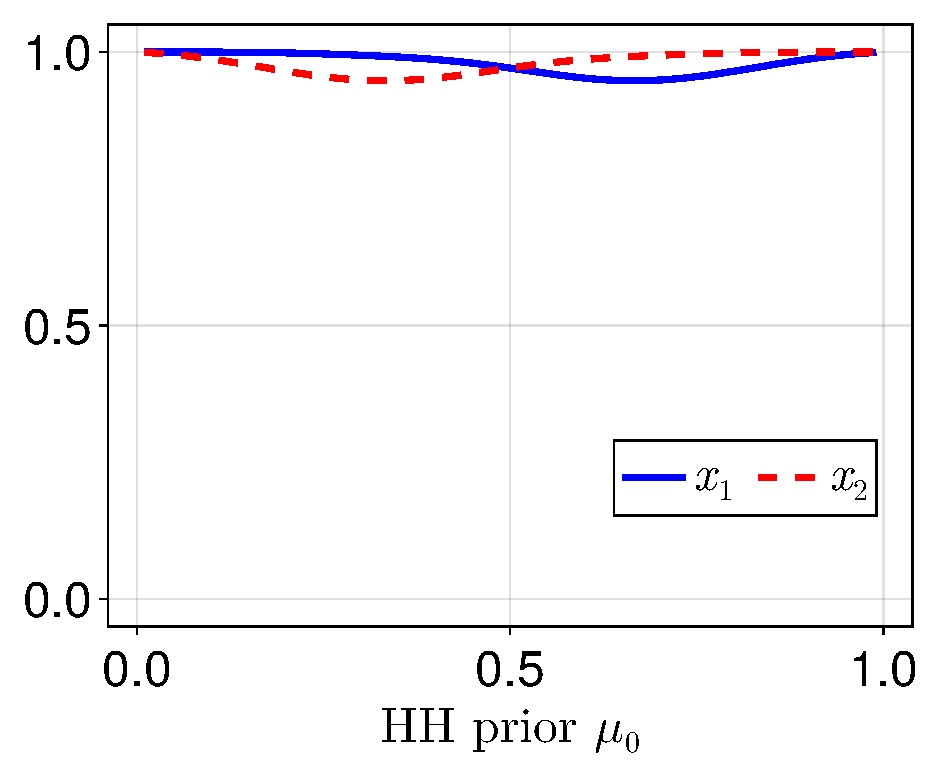
\includegraphics[width=0.49\textwidth]{figures/V8/γ_10/fig_optimal_π_across_μ_0_ω_1_1_ω_2_-1_δ_0.5_.pdf}
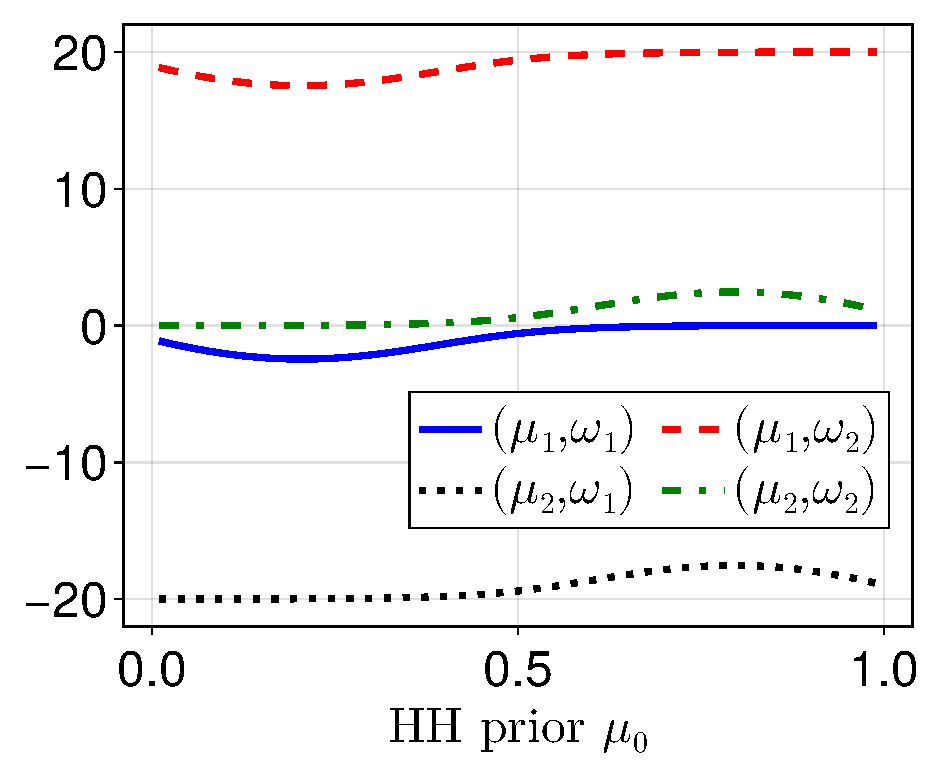
\includegraphics[width=0.49\textwidth]{figures/V8/γ_10/fig_posterior_across_μ_0_ω_1_1_ω_2_-1_δ_0.5_.pdf}
\caption{Comparative statics for $\mu_0$ varying from 0 to 1, holding fixed all other parameters as in the benchmark.}
\label{Figure1}
\end{figure}

As Figure \ref{Figure1} shows, when HHs are either too optimistic or pessimistic, the effect on the information design is limited compared to the benchmark. CB's strategy is dominated by condition \eqref{threshold} dictating that, in the current scenario, inflation surprise is excessive and, thus, it is best for CB to remove uncertainty, although this will generate an unemployment gap. For instance, when HHs are mildly pessimistic (e.g., $\mu_0=0.7$), CB sets $x_2=1$ and $x_1$ smaller but close to 1. In other words, CB reveals whenever the negative shock (i.e., $\omega_1$) happens, while leaving some residual uncertainty on the positive shock (i.e., $\omega_2)$. Generalizing, CB focuses on eliminating the inflation surprise when the most plausible shock from the perspective of HHs realizes. This is likely due to the higher entropy cost associated with revealing the least plausible shock. Indeed, CB's intervention is not fully informative because of the presence of inattentive HHs. Increasing (decreasing) the share of inattentive HHs has the obvious effect of decreasing (increasing) the precision of CB's recommendations. This effect is asymmetric when HHs beliefs are not neutral, penalizing precision under the least plausible shock. See Figures \ref{FigureA1} and \ref{FigureA2} in the Appendix.

\begin{figure}[H]
\centering
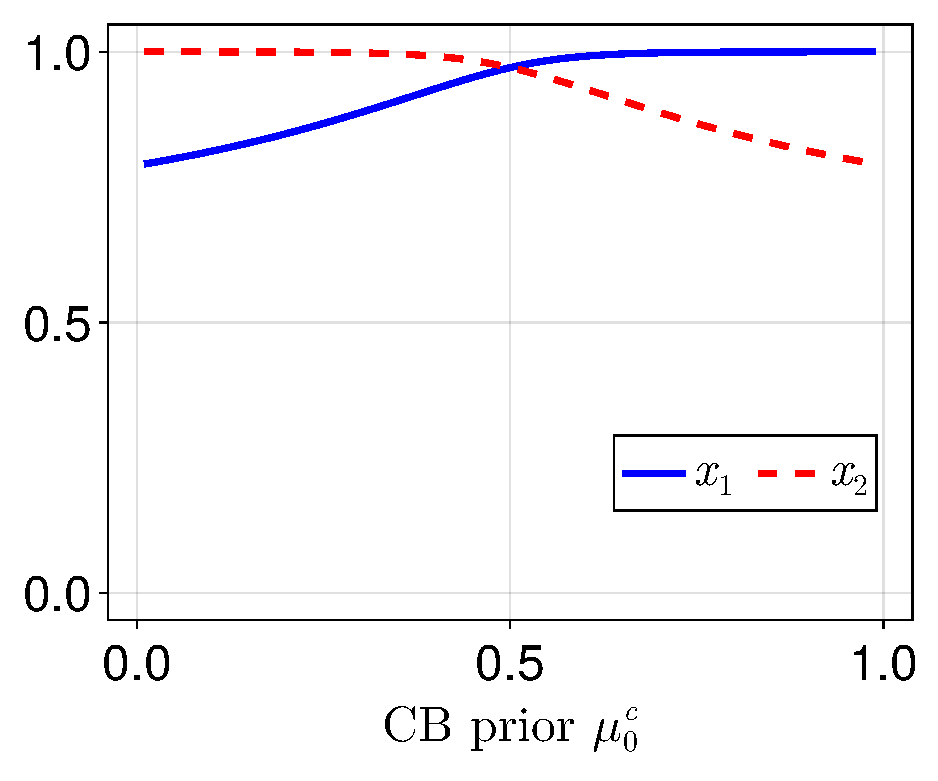
\includegraphics[width=0.49\textwidth]{figures/V8/γ_10/fig_optimal_π_across_μ_0_c_ω_1_1_ω_2_-1_δ_0.5_.pdf}
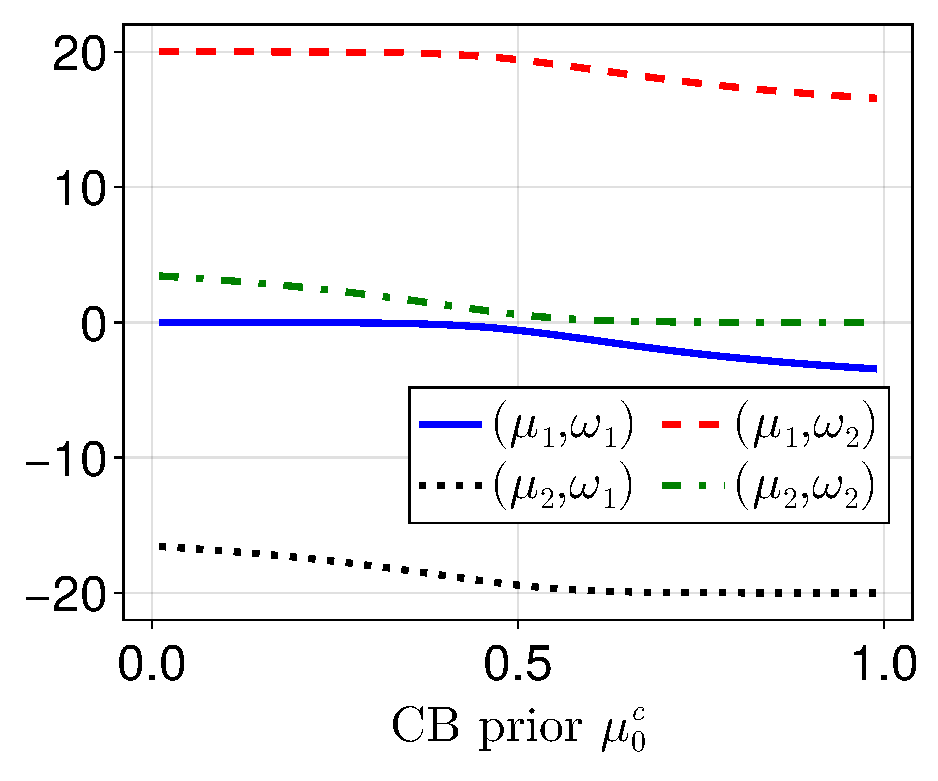
\includegraphics[width=0.49\textwidth]{figures/V8/γ_10/fig_posterior_across_μ_0_c_ω_1_1_ω_2_-1_δ_0.5_.pdf}
\caption{Comparative statics for $\mu_0^c$ varying from 0 to 1, holding fixed all other parameters as in the benchmark.}
\label{Figure2}
\end{figure}

Figure \ref{Figure2} shows the effect of superior knowledge by the CB. In contrast to the effect of HHs optimism or pessimism, CB sacrifices precision of its recommendations concerning the shock that CB considers most plausible. The difference comes from the magnitude of inflation surprise, which is constant here, since $\mu_0=\frac{1}{2}$, whereas $\mu_0^c$ varies. For instance, when $\mu_0^c=0.7$, then $x_1=1$ whereas $x_2$ is smaller than 1. Equivalently, if CB believes a negative shock (i.e., $\omega_1$) to be more plausible, it will reveal whenever a positive shock (i.e., $\omega_2$) happens, while keeping some uncertainty on the negative shock. Indeed, given the presence of inattentive HHs, CB cannot completely eliminate inflation surprise. As before, this effect becomes more (less) prominent when the share of inattentive HHs increases (decreases). See Figures \ref{FigureA3} and \ref{FigureA4} in the Appendix.

\paragraph{Unemployment Shocks}
We are now interested in how asymmetric shocks come into play with belief heterogeneity, particularly the roles of shock magnitude and asymmetry. To this end, in contrast to the benchmark, where we consider $(\omega_1,\omega_2)=(1,-1)$, we further examine the effects of two extra cases: $(\omega_1,\omega_2)=(2,-2)$ and $(\omega_1,\omega_2)=(2,-1)$. The first case aims to study the role of shock magnitude, while the second checks the role of shock asymmetry. We then vary each HHs and CB priors at a time for the two cases and follow the same convention for reporting results. In other words, we redo the previous exercises with different shock combinations. The results are that neither shocks magnitude nor asymmetry play a significant role.
See Figures \ref{FigureA5}-\ref{FigureA8} in the Appendix. Remarkably, shocks play a role in the determining a discontinuity point in information design. See condition \eqref{threshold} and the results of the next section. Finally, we investigate how the effect of magnitude and asymmetry of shocks interact with the share of inattentive HHs. Our analysis confirms that shocks have only a limited impact on the precision of CB's information. See Figures \ref{FigureA9}-\ref{FigureA16} in the Appendix.


\subsection{Flatter Phillips Curve}
The flattened Phillips curve has become the new paradigm for interpreting the relationship between unemployment and inflation in recent years. It means the curve's inflation sensitivity $\gamma$ has approached one. This issue has become a major concern for policymakers on the effectiveness of monetary policy, especially while guiding the inflation expectation of market participants. To evaluate how such structural change affects the previous conclusions, we redo the same exercises as above with $\gamma=1$. Interestingly, when $\gamma=1$, this corresponds to the case when $4\omega > \gamma (\nu_1 + \nu_2)$, captured in our Propositions \ref{Prop1}-\ref{Prop3}. Remarkably, our theoretical prediction for this scenario is that CB provides no information (or, equivalently, designs uninformative signals). This happens because the inflation surprise is relatively small and, in a condition of uncertainty by HHs, helps to reduce the impact of unemployment shocks. 

\paragraph{Heterogeneous Beliefs}
As before, we focus our analysis on the possibility that HHs and CB hold different prior beliefs. As Figure \ref{Figure3} shows, CB intervenes if HHs are either too optimistic or too pessimistic. In particular, in our benchmark where $\mu_0=\mu_0^c=\frac{1}{2}$, the inflation surprise exactly compensates for the shocks, thus implying a zero unemployment gap. This is the best scenario for the central bank and there is no reason to intervene. Consider, for instance, the possibility that HHs are instead too pessimistic (that is, $\mu_0\to 1$). There exists a threshold value of $\mu_0$ such that above it CB finds it optimal to send informative reports. In particular, above such threshold, $x_2=1$, implying that CB commits to revael to HHs whenever the negative shock (i.e., $\omega_1$) realizes. Why? Note that, as $\mu_0\to 1$, the inflation surprise becomes excessive in the case of a positive shock (i.e., $\omega_2$), whereas it is insufficient in the event of a negative shock. When this imbalance grows excessively, CB corrects it using signal $s_2$, which brings the inflation surprise closer to the optimal level. This comes at the cost of increasing the loss associated to $s_1$. Nevertheless, this is optimal for CB because $s_2$ occurs more often than $s_1$. Generalizing, CB responds to excessive optimism or pessimism by HHs inducing the optimal inflation surprise when the shock that HHs consider the least plausible realizes.

\begin{figure}[H]
\centering
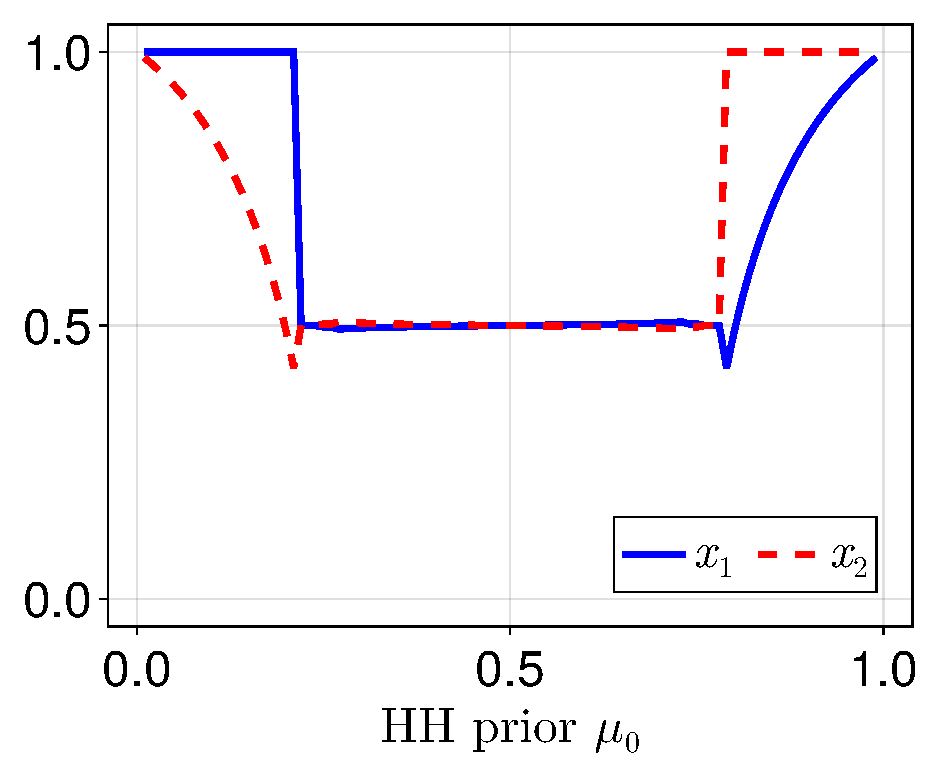
\includegraphics[width=0.49\textwidth]{figures/V8/γ_1/fig_optimal_π_across_μ_0_ω_1_1_ω_2_-1_δ_0.5_.pdf}
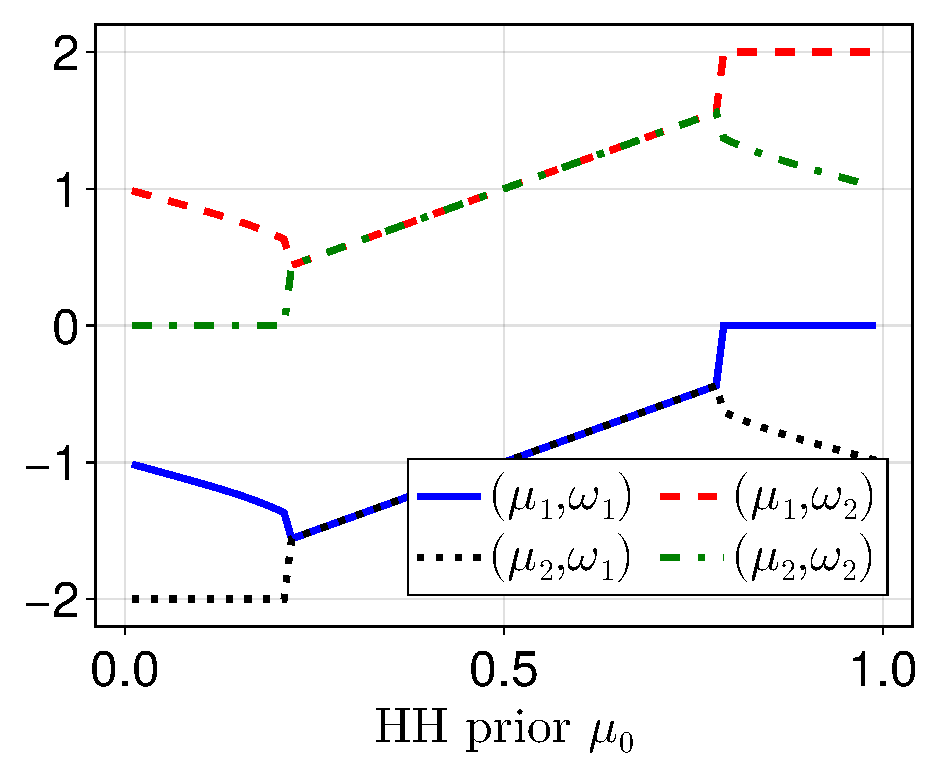
\includegraphics[width=0.49\textwidth]{figures/V8/γ_1/fig_posterior_across_μ_0_ω_1_1_ω_2_-1_δ_0.5_.pdf}
\caption{Comparative statics for $\mu_0$ varying from 0 to 1, holding fixed all other parameters as in the benchmark.}
\label{Figure3}
\end{figure}

Instead, as Figure \ref{Figure4} shows, a superior knowledge by CB has no impact on information design. The reason, as mentioned before, is the fact that given $\mu_0=\frac{1}{2}$ inflation surprise is already at its optimal level. Thus, CB finds it optimal to provide no further information.

\begin{figure}[H]
\centering
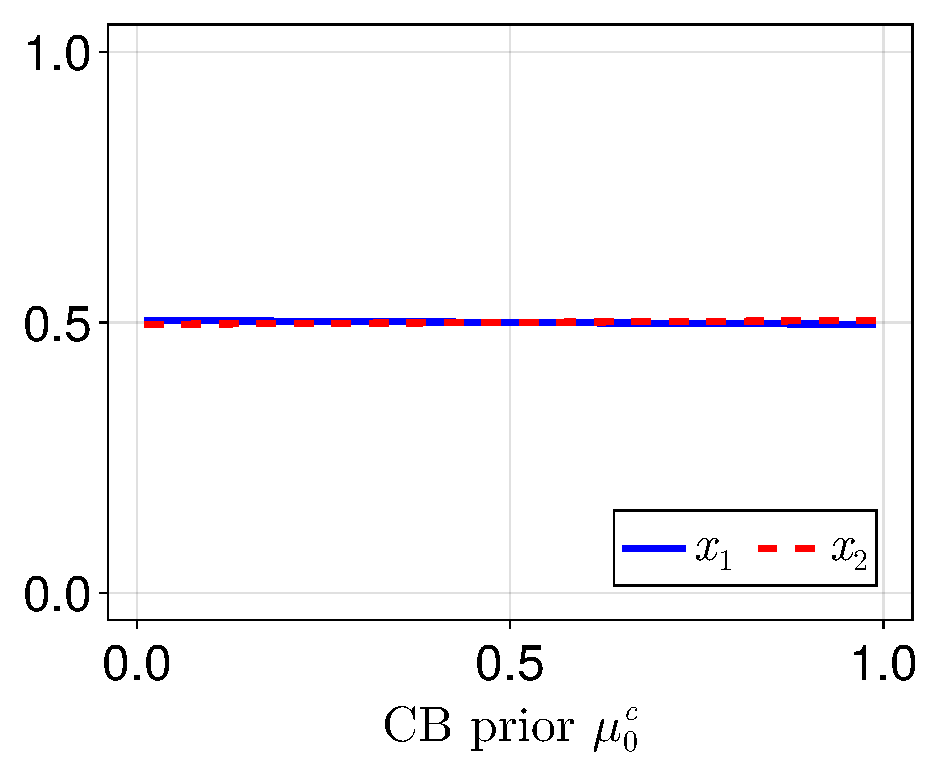
\includegraphics[width=0.49\textwidth]{figures/V8/γ_1/fig_optimal_π_across_μ_0_c_ω_1_1_ω_2_-1_δ_0.5_.pdf}
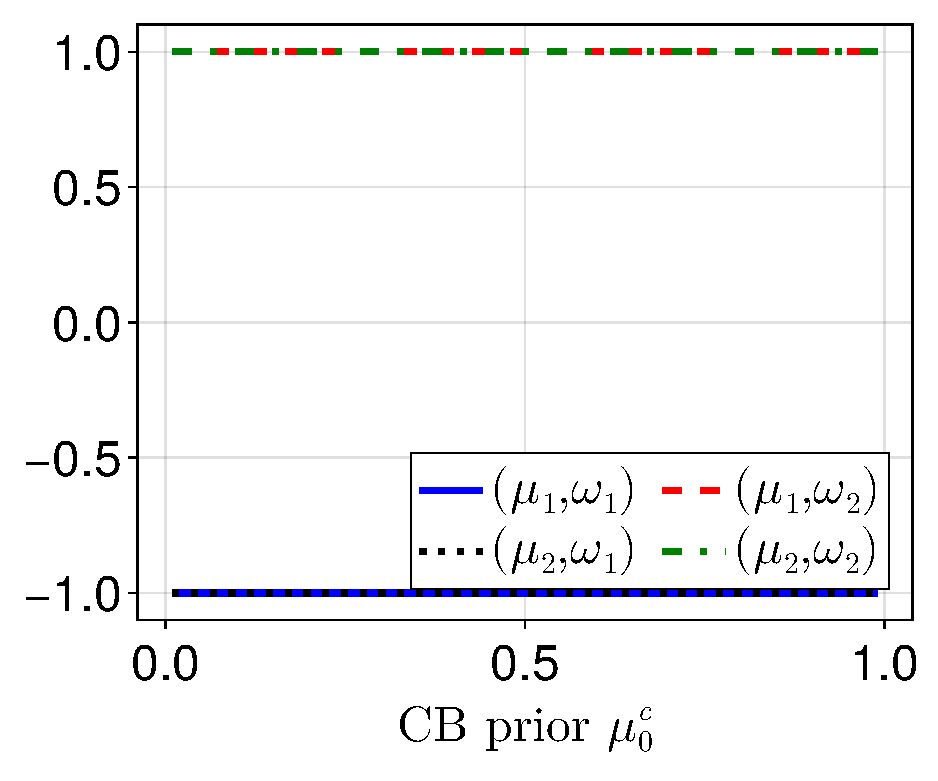
\includegraphics[width=0.49\textwidth]{figures/V8/γ_1/fig_posterior_across_μ_0_c_ω_1_1_ω_2_-1_δ_0.5_.pdf}
\caption{Comparative statics for $\mu_0^c$ varying from 0 to 1, holding fixed all other parameters as in the benchmark.}
\label{Figure4}
\end{figure}

\paragraph{Unemployment Shocks}
The magnitude and asymmetry of unemployment shocks change CB's response because they impact the optimality of inflation surprise in the benchmark. In particular, when $\mu_0=\frac{1}{2}$, the inflation surprise is insufficient, independently on the shock. Varying $\mu_0$ brings inflation surprise closer to the optimal level for one shock, but meanwhile away from the optimal level for the other shock. Information design cannot help CB in this scenario. See Figures \ref{FigureA17}-\ref{FigureA20} in the Appendix.


\paragraph{Share of Inattentive Households}
In this case, inattention does not play any significant role, neither alone nor in interaction with the magnitude and asymmetry of unemployment shocks. See Figures \ref{FigureA21}-\ref{FigureA32} in the Appendix.

\section{Optimal Flexibility in Asymmetric Scenarios} 

\section{Conclusion}

\newpage
\bibliographystyle{ecta}
\bibliography{references}

\appendix

\section{Mathematical details}
\label{math}
We denote with $x_1=\pi(s_1|\omega_1)$ and $x_2=\pi(s_2|\omega_2)$. It follows that:
\begin{align}
    \mu_1 & = \frac{x_1\mu_0}{x_1\mu_0 + (1-x_2)(1-\mu_0)} \\
    \mu_2 & = \frac{(1-x_1)\mu_0}{(1-x_1)\mu_0 + x_2(1-\mu_0)}\\
    \frac{\partial \mu_1}{\partial x_1} & =\frac{\mu_0(1-\mu_0)(1-x_2)}{[x_1\mu_0+(1-x_2)(1-\mu_0)]^2}\\
    \frac{\partial \mu_2}{\partial x_1} & =\frac{-\mu_0(1-\mu_0)x_2}{[(1-x_1)\mu_0+x_2(1-\mu_0)]^2}\\
    \frac{\partial \mu_1}{\partial x_2} & =\frac{\mu_0(1-\mu_0)x_1}{[x_1\mu_0+(1-x_2)(1-\mu_0)]^2}\\
    \frac{\partial \mu_2}{\partial x_2} & =\frac{-\mu_0(1-\mu_0)(1-x_1)}{[(1-x_1)\mu_0+x_2(1-\mu_0)]^2}
\end{align}
\paragraph{Proof of Proposition \ref{Prop1}}
The F.O.C. when $\delta=0$ are:
\begin{small}
\begin{eqnarray}
\label{focx1gen2}
    \begin{split}
        \mu_0^c\Bigg[(\omega_1-\gamma(\nu_1+\nu_2)(1-\mu_1))^2+2x_1(\omega_1-\gamma(\nu_1+\nu_2)(1-\mu_1))\gamma(\nu_1+\nu_2)\frac{\partial \mu_1}{\partial x_1}+ & \\
        -(\omega_1-\gamma(\nu_1+\nu_2)(1-\mu_2))^2+2(1-x_1)(\omega_1-\gamma(\nu_1+\nu_2)(1-\mu_2))\gamma(\nu_1+\nu_2)\frac{\partial \mu_2}{\partial x_1}\Bigg]+ &\\
        2\gamma(\nu_1+\nu_2)(1-\mu_0^c)\left[x_2(\omega_2+\gamma(\nu_1+\nu_2)\mu_2)\frac{\partial \mu_2}{\partial x_1}+(1-x_2)(\omega_2+\gamma(\nu_1+\nu_2)\mu_1)\frac{\partial \mu_1}{\partial x_1}\right] & =0
    \end{split} \\ 
    \label{focx2gen2}
    \begin{split}
    2\gamma(\nu_1+\nu_2)\mu_0^c\left[x_1(\omega_1-\gamma(\nu_1+\nu_2)(1-\mu_1))\frac{\partial \mu_1}{\partial x_2}+(1-x_1)(\omega_1-\gamma(\nu_1+\nu_2)(1-\mu_2))\frac{\partial \mu_2}{\partial x_2}\right]+ &\\
    (1-\mu_0^c)\Bigg[(\omega_2+\gamma(\nu_1+\nu_2)\mu_2)^2+2x_2(\omega_2+\gamma(\nu_1+\nu_2)\mu_2)\gamma(\nu_1+\nu_2)\frac{\partial \mu_2}{\partial x_2}+ & \\
    -(\omega_2+\gamma(\nu_1+\nu_2)\mu_1)^2+2(1-x_2)(\omega_2+\gamma(\nu_1+\nu_2)\mu_1)\gamma(\nu_1+\nu_2)\frac{\partial \mu_1}{\partial x_2}\Bigg] & =0
    \end{split}
\end{eqnarray}
\end{small}
Applying assumptions \ref{Ass3}-\ref{Ass4}, the F.O.C.s becomes symmetric. Thus, we consider symmetric solutions where $x_1=x_2=x$ and the result follows.
\paragraph{Proof of Proposition \ref{Prop2}}
In the first stage, the utility of CB is:
\begin{equation*}
u=\left\{\begin{array}{cc}
   -\omega^2  & \omega<\frac{\gamma}{4} (\nu_1+\nu_2)\\
   -\left(\omega-\frac{\gamma}{2}(\nu_1+\nu_2)\right)^2  & \omega\geq\frac{\gamma}{4} (\nu_1+\nu_2)
\end{array}\right.
\end{equation*}
Under assumptions \ref{Ass3}-\ref{Ass4}, the CB's problem \eqref{minproblem2} becomes:
\begin{equation}
    \begin{split}
    \min_{\{\nu_1,\nu_2\}} \ & \ \left(\omega-\frac{\gamma}{2}(\nu_1+\nu_2)\right)^2
    +\frac{\alpha}{2}(\nu_1^2+\nu_2^2)
    \end{split}
\end{equation}
subject to $\omega\geq\frac{\gamma}{4} (\nu_1+\nu_2)$. The F.O.C.s are:
\begin{eqnarray}
2\left(\omega-\frac{\gamma}{2}(\nu_1+\nu_2)\right)\left(-\frac{\gamma}{2}\right)+\alpha \nu_1=0\\
2\left(\omega-\frac{\gamma}{2}(\nu_1+\nu_2)\right)\left(-\frac{\gamma}{2}\right)+\alpha \nu_2=0
\end{eqnarray}
Since the F.O.C.s are symmetric, the solution is symmetric:
\begin{equation}
    \nu_1=\nu_2=\nu=\left(\frac{\gamma}{\gamma^2+\alpha}\right)\omega
\end{equation}
The problem is correctly specified since
\begin{equation}
    \omega\geq\frac{\gamma}{4} (\nu_1+\nu_2)=\left(\frac{\gamma^2}{2(\gamma^2+\alpha)}\right)\omega 
\end{equation}
Note that, if we assume $\omega<\frac{\gamma}{4} (\nu_1+\nu_2)$, the optimal solution is $\nu_1=\nu_2=0$, which produces a contradiction.
\paragraph{Proof of Proposition \ref{Prop3}}
The F.O.C. when $\delta\neq 0$ are:
\begin{small}
\begin{equation}
    \begin{split}
        \delta c^\prime(\pi)\Bigg\{\mu_0^c\left[\omega_1-\gamma(\nu_1+\nu_2)(1-\mu_0)\right]^2+(1-\mu_0^c)\left[\omega_2+\gamma(\nu_1+\nu_2)\mu_0\right]^2\Bigg\}+ &\\
        -\delta c^\prime(\pi)\Bigg\{\mu_0^c\bigg[\pi(s_1|\omega_1)(\omega_1-\gamma (\nu_1+\nu_2) (1-\mu_1))^2+\pi(s_2|\omega_1)(\omega_1-\gamma (\nu_1+\nu_2) (1-\mu_2))^2\bigg]+ & \\
        +(1-\mu_0^c)\bigg[\pi(s_2|\omega_2)(\omega_2+\gamma (\nu_1+\nu_2) \mu_2)^2+\pi(s_1|\omega_2)(\omega_2+\gamma (\nu_1+\nu_2) \mu_1)^2 \bigg]\Bigg\}+ & \\
        +[1-\delta c(\pi)]\Bigg\{\mu_0^c\Bigg[(\omega_1-\gamma(\nu_1+\nu_2)(1-\mu_1))^2+2x_1(\omega_1-\gamma(\nu_1+\nu_2)(1-\mu_1))\gamma(\nu_1+\nu_2)\frac{\partial \mu_1}{\partial x_1}+ & \\
        -(\omega_1-\gamma(\nu_1+\nu_2)(1-\mu_2))^2+2(1-x_1)(\omega_1-\gamma(\nu_1+\nu_2)(1-\mu_2))\gamma(\nu_1+\nu_2)\frac{\partial \mu_2}{\partial x_1}\Bigg]+ &\\
        +2\gamma(\nu_1+\nu_2)(1-\mu_0^c)\left[x_2(\omega_2+\gamma(\nu_1+\nu_2)\mu_2)\frac{\partial \mu_2}{\partial x_1}+(1-x_2)(\omega_2+\gamma(\nu_1+\nu_2)\mu_1)\frac{\partial \mu_1}{\partial x_1}\right]\Bigg\} & =0
    \end{split} 
\end{equation}
\begin{equation}
    \begin{split}
    \delta c^\prime(\pi)\Bigg\{\mu_0^c\left[\omega_1-\gamma(\nu_1+\nu_2)(1-\mu_0)\right]^2+(1-\mu_0^c)\left[\omega_2+\gamma(\nu_1+\nu_2)\mu_0\right]^2\Bigg\}+ &\\
    -\delta c^\prime(\pi)\Bigg\{\mu_0^c\bigg[\pi(s_1|\omega_1)(\omega_1-\gamma (\nu_1+\nu_2) (1-\mu_1))^2+\pi(s_2|\omega_1)(\omega_1-\gamma (\nu_1+\nu_2) (1-\mu_2))^2\bigg]+ & \\
    +(1-\mu_0^c)\bigg[\pi(s_2|\omega_2)(\omega_2+\gamma (\nu_1+\nu_2) \mu_2)^2+\pi(s_1|\omega_2)(\omega_2+\gamma (\nu_1+\nu_2) \mu_1)^2 \bigg]\Bigg\}+ & \\
    +[1-\delta c(\pi)]\Bigg\{
    (1-\mu_0^c)\Bigg[(\omega_2+\gamma(\nu_1+\nu_2)\mu_2)^2+2x_2(\omega_2+\gamma(\nu_1+\nu_2)\mu_2)\gamma(\nu_1+\nu_2)\frac{\partial \mu_2}{\partial x_2}+ & \\
    -(\omega_2+\gamma(\nu_1+\nu_2)\mu_1)^2+2(1-x_2)(\omega_2+\gamma(\nu_1+\nu_2)\mu_1)\gamma(\nu_1+\nu_2)\frac{\partial \mu_1}{\partial x_2}\Bigg]+ & \\
    +2\gamma(\nu_1+\nu_2)\mu_0^c\left[x_1(\omega_1-\gamma(\nu_1+\nu_2)(1-\mu_1))\frac{\partial \mu_1}{\partial x_2}+(1-x_1)(\omega_1-\gamma(\nu_1+\nu_2)(1-\mu_2))\frac{\partial \mu_2}{\partial x_2}\right]\Bigg\} & =0
    \end{split}
\end{equation}
\end{small}
where the marginal cost of information $c^\prime(\pi)$ has the following expression:
\begin{align}
    c^\prime(\pi) & = -\chi \sum_{j=1,2} \left[\frac{\partial \tau_{j}}{\partial x_k}H(\mu_j) + \tau_{j}\frac{\partial H(\mu_j)}{\partial x_k}\right].
\end{align}
Applying assumptions \ref{Ass3}-\ref{Ass4}, the F.O.C.s becomes symmetric. Thus, we consider symmetric solutions where $x_1=x_2=x$.
It follows that the solution to the CB's information design problem solves the following condition:
    \begin{equation}
    \label{focdeltanonzero}
        \gamma(\nu_1+\nu_2)[4\omega-\gamma(\nu_1+\nu_2)]\left\{[1-\delta c(\pi)](2x-1)+2\delta c^\prime(\pi)\left[x(1-x)-\frac{1}{4}\right]\right\}=0
    \end{equation}
    where
    \begin{eqnarray}
        c(\pi)=\chi \left[\ln(2)+x\ln(x)+(1-x)\ln(1-x)\right] \\
        c^\prime(\pi)=\frac{\chi}{2}\left[\ln\left(x\right)-\ln(1-x)\right]
    \end{eqnarray}
    Since
    \begin{eqnarray}
        2\delta c^\prime(\pi)\left[x(1-x)-\frac{1}{4}\right]\leq 0 \quad \forall x\in\left[\frac{1}{2},1\right] \\
        \lim_{x\to 1}2\delta c^\prime(\pi)\left[x(1-x)-\frac{1}{4}\right]=-\infty \\
        \lim_{x\to\frac{1}{2}}[1-\delta c(\pi)](2x-1)+2\delta c^\prime(\pi)\left[x(1-x)-\frac{1}{4}\right]=0
    \end{eqnarray}
    If there exists a solution to \eqref{focdeltanonzero}, then it must be a maximum point, provided that $4\omega-\gamma(\nu_1+\nu_2)\geq0$. Therefore, CB's problem has a corner solution: either $x=\frac{1}{2}$ or $x=1$. CB's utility when $x=\frac{1}{2}$ is
    \begin{equation}
        u_{x=\frac{1}{2}}=-\left[\omega-\frac{\gamma}{2}(\nu_1+\nu_2)\right]^2
    \end{equation}
    whereas CB's utility when $x=1$ is
    \begin{equation}
        u_{x=1}=-\delta\left[\omega-\frac{\gamma}{2}(\nu_1+\nu_2)\right]^2-(1-\delta)\omega^2
    \end{equation}
Comparing these two, we observe that CB's utility is higher with $x=\frac{1}{2}$ if and only if
\begin{equation}
\label{constraintomega}
    \left[\omega-\frac{\gamma}{2}(\nu_1+\nu_2)\right]^2\leq \omega^2 \iff \omega\geq \frac{\gamma}{4}(\nu_1+\nu_2)
\end{equation}
The optimal flexibility given $x=\frac{1}{2}$ is, as before:
\begin{equation}
\label{optflex}
    \nu_1=\nu_2=\nu=\left(\frac{\gamma}{\gamma^2+\alpha}\right)\omega
\end{equation}
which satisfies \eqref{constraintomega}. When \eqref{constraintomega} does not hold, there can be an interior solution to \eqref{focdeltanonzero}. CB's utility with a generic symmetric solution $x\in\left[\frac{1}{2},1\right]$ is:
\begin{equation}
    \begin{split}
        u_{x}= & \, -\delta c(\pi)\left[\omega-\frac{\gamma}{2}(\nu_1+\nu_2)\right]^2+\\
        & -(1-\delta c(\pi))\left[x(\omega-\gamma(\nu_1+\nu_2)(1-x))^2+(1-x)(\omega-\gamma(\nu_1+\nu_2)x)^2\right]
    \end{split}
\end{equation}
We verify that $u_x\geq u_{x=\frac{1}{2}}$ if and only if \eqref{constraintomega} does not hold. Following \eqref{focdeltanonzero}, the optimal precision of information $x$ solves:
\begin{equation}
    [1-\delta\chi\ln(2)](2x-1)+\delta\chi \left[\ln(x)\left(2x-3x^2-\frac{1}{4}\right)+\ln(1-x)\left(3x^2-4x+\frac{5}{4}\right)\right]=0
\end{equation}
There exists a threshold value $\hat{\delta}$ such that $x=1$ for any $\delta\leq \hat{\delta}$, whereas $x\in\left(\frac{1}{2},1\right)$ for any $\delta>\hat{\delta}$. Remarkably, the solution $x$ to \eqref{focdeltanonzero} does not depend on $\nu_1$ and $\nu_2$. The CB's problem in the first stage is:
\begin{equation}
    \begin{split}
    \min_{\{\nu_1,\nu_2\}} \ & \ -u_x
    +\frac{\alpha}{2}(\nu_1^2+\nu_2^2)
    \end{split}
\end{equation}
The corresponding F.O.C.s are:
\begin{eqnarray}
2\delta c(\pi)\left(\omega-\frac{\gamma}{2}(\nu_1+\nu_2)\right)\left(-\frac{\gamma}{2}\right)+2[1-\delta c(\pi)]\left[x(1-x)(2\omega-\gamma(\nu_1+\nu_2))\right](-\gamma)+\alpha \nu_1=0\\
2\delta c(\pi)\left(\omega-\frac{\gamma}{2}(\nu_1+\nu_2)\right)\left(-\frac{\gamma}{2}\right)+2[1-\delta c(\pi)]\left[x(1-x)(2\omega-\gamma(\nu_1+\nu_2))\right](-\gamma)+\alpha \nu_2=0
\end{eqnarray}
The F.O.C.s are symmetric. Thus, $\nu_1=\nu_2=\nu$, which implies:
\begin{equation}
\label{focsymmetricv}
    -\gamma\delta c(\pi)\left(\omega-\gamma \nu\right)-4\gamma[1-\delta c(\pi)]\left[x(1-x)(\omega-\gamma \nu)\right]+\alpha \nu=0
\end{equation}
Therefore, the optimal flexibility $\hat{\nu}$ solving \eqref{focsymmetricv} is:
\begin{equation}
    \hat{\nu}=\left(\frac{\gamma \left\{4x(1-x)+\delta c(\pi)[1-4x(1-x)]\right\}}{\gamma^2\left\{4x(1-x)+\delta c(\pi)[1-4x(1-x)] \right\}+\alpha }\right)\omega
\end{equation}
When $\nu_1=\nu_2=\hat{\nu}$, the condition \eqref{constraintomega} holds, thus contradicting the initial assumption. We conclude that a partially or fully informative $\pi$ cannot be part of the equilibrium path. For CB, it is optimal to give flexibility $\nu$ as in \eqref{optflex} and, then, provide no information.

\section{Numerical Exercises}

\begin{figure}[H]
\centering
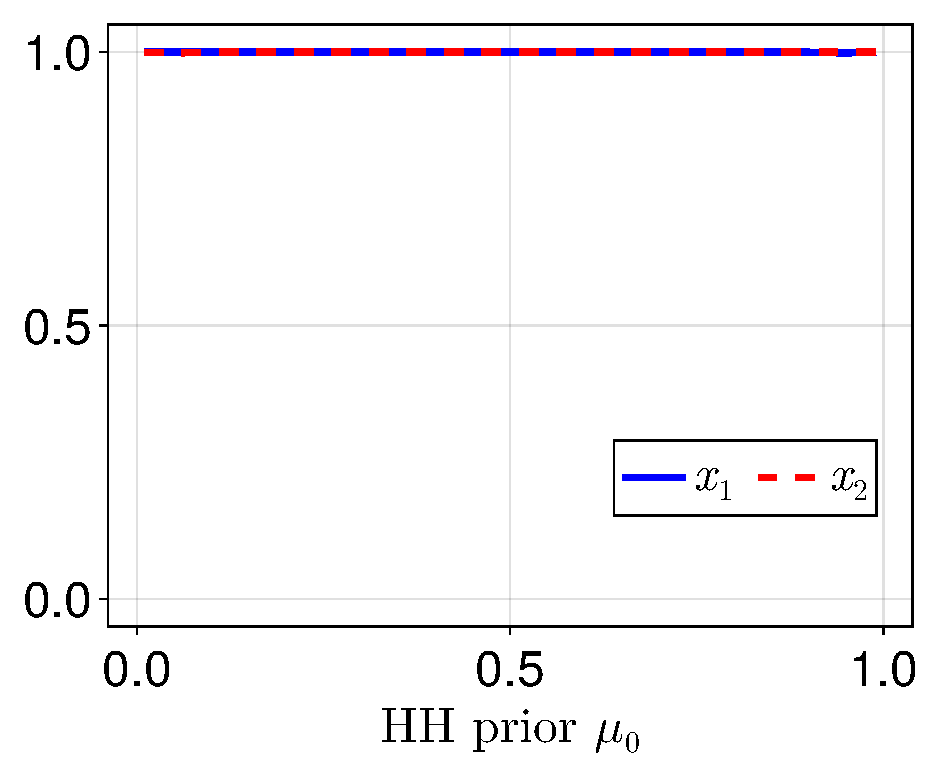
\includegraphics[width=0.49\textwidth]{figures/V8/γ_10/fig_optimal_π_across_μ_0_ω_1_1_ω_2_-1_δ_0.0_.pdf}
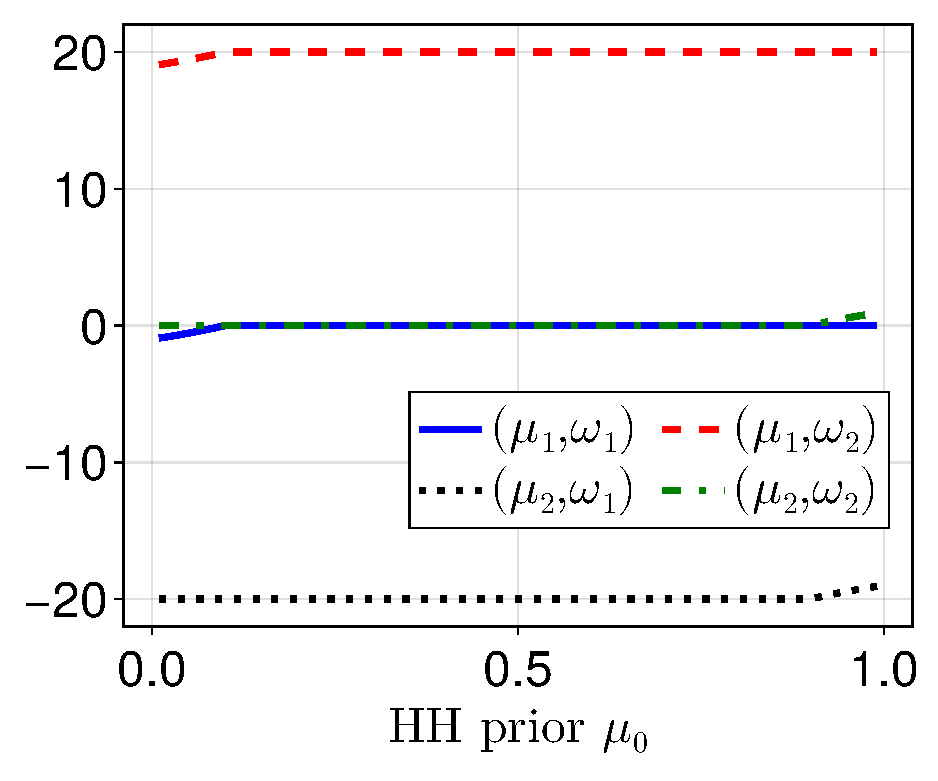
\includegraphics[width=0.49\textwidth]{figures/V8/γ_10/fig_posterior_across_μ_0_ω_1_1_ω_2_-1_δ_0.0_.pdf}
\caption{Comparative statics for $\mu_0$, when $\delta=0$, holding fixed all other parameters as in the benchmark.}
\label{FigureA1}
\end{figure}

\begin{figure}[H]
\centering
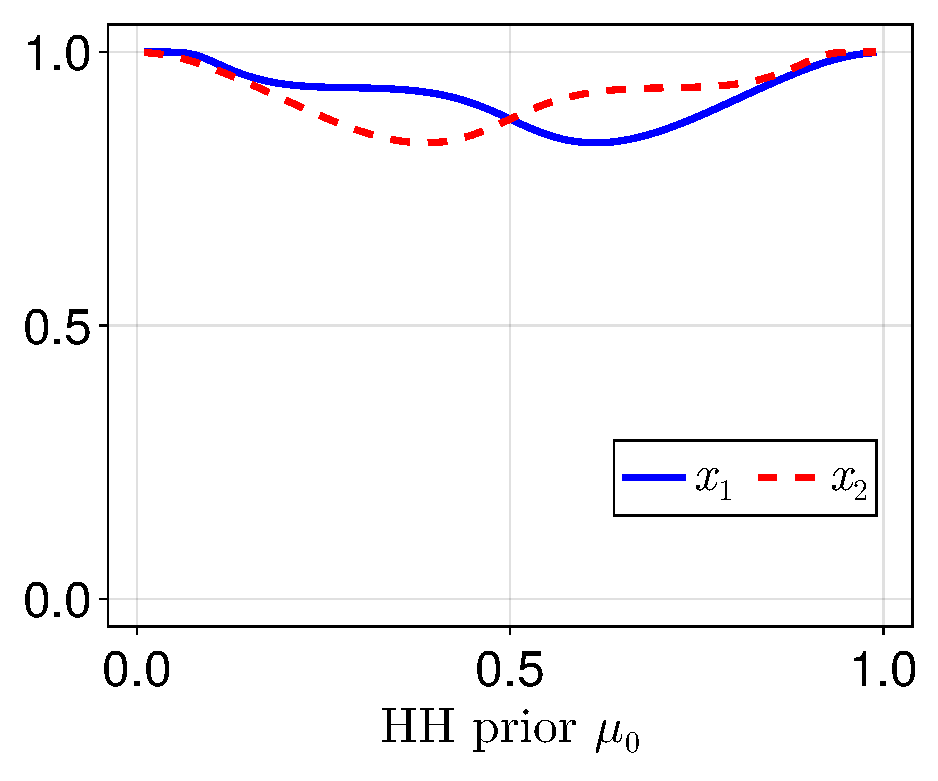
\includegraphics[width=0.49\textwidth]{figures/V8/γ_10/fig_optimal_π_across_μ_0_ω_1_1_ω_2_-1_δ_1.0_.pdf}
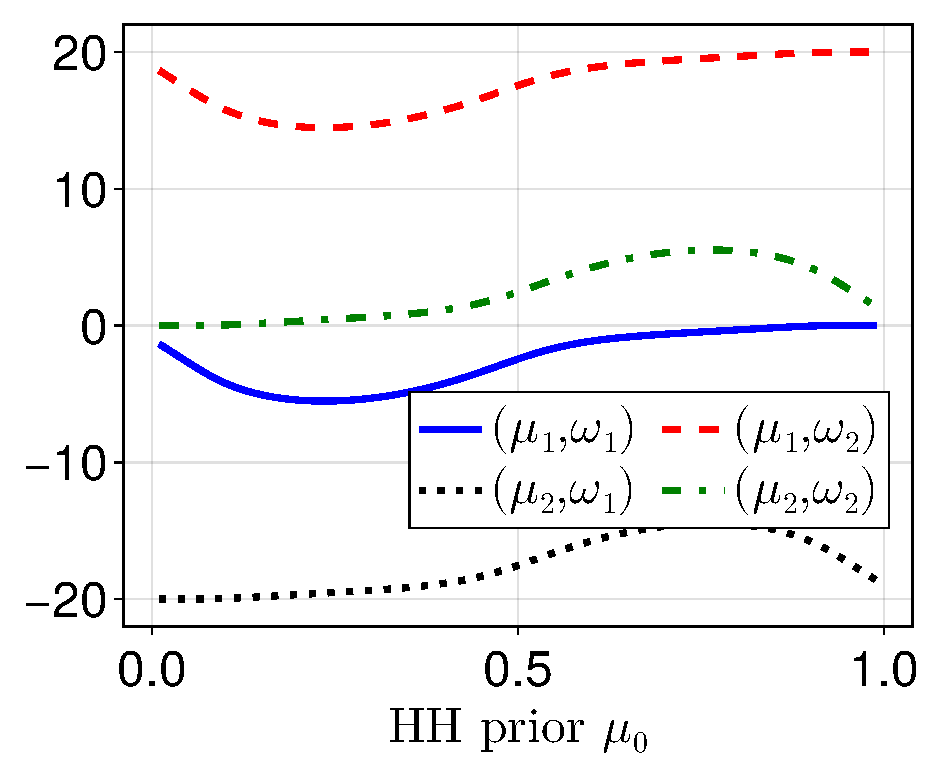
\includegraphics[width=0.49\textwidth]{figures/V8/γ_10/fig_posterior_across_μ_0_ω_1_1_ω_2_-1_δ_1.0_.pdf}
\caption{Comparative statics for $\mu_0$, when $\delta=1$, holding fixed all other parameters as in the benchmark.}
\label{FigureA2}
\end{figure}

\begin{figure}[H]
\centering
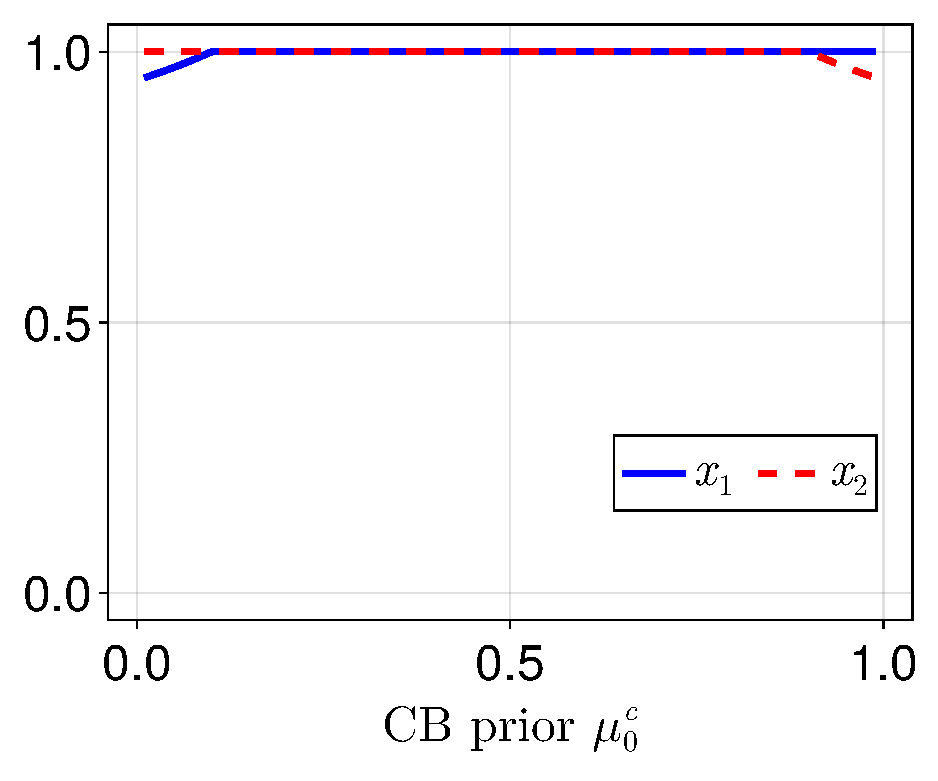
\includegraphics[width=0.49\textwidth]{figures/V8/γ_10/fig_optimal_π_across_μ_0_c_ω_1_1_ω_2_-1_δ_0.0_.pdf}
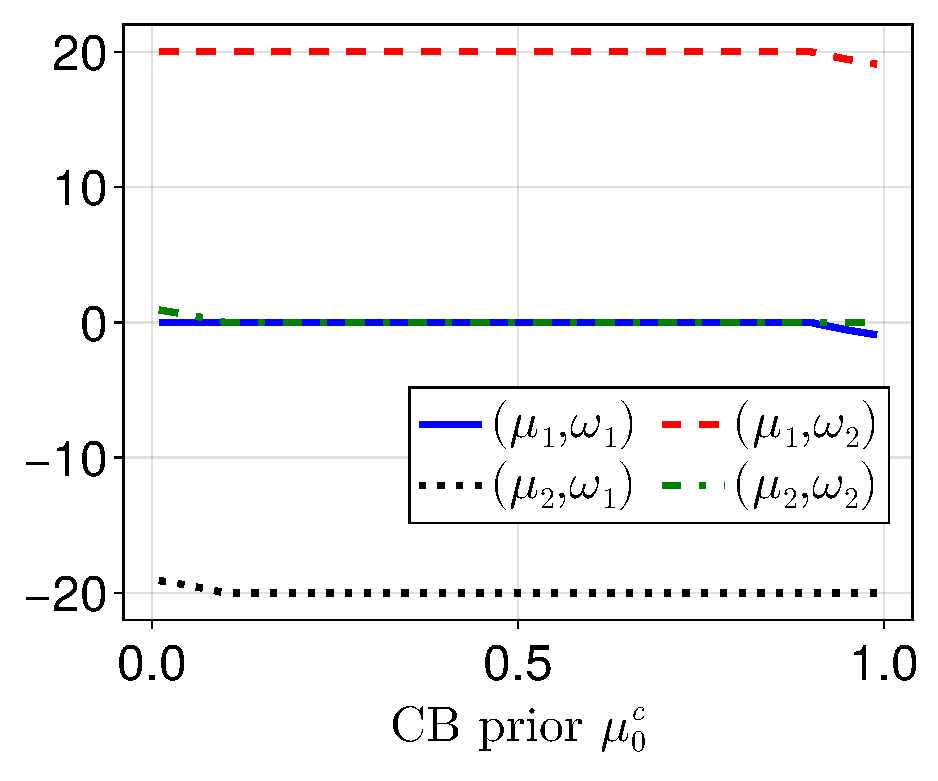
\includegraphics[width=0.49\textwidth]{figures/V8/γ_10/fig_posterior_across_μ_0_c_ω_1_1_ω_2_-1_δ_0.0_.pdf}
\caption{Comparative statics for $\mu_0^c$, when $\delta=0$, holding fixed all other parameters as in the benchmark.}
\label{FigureA3}
\end{figure}

\begin{figure}[H]
\centering
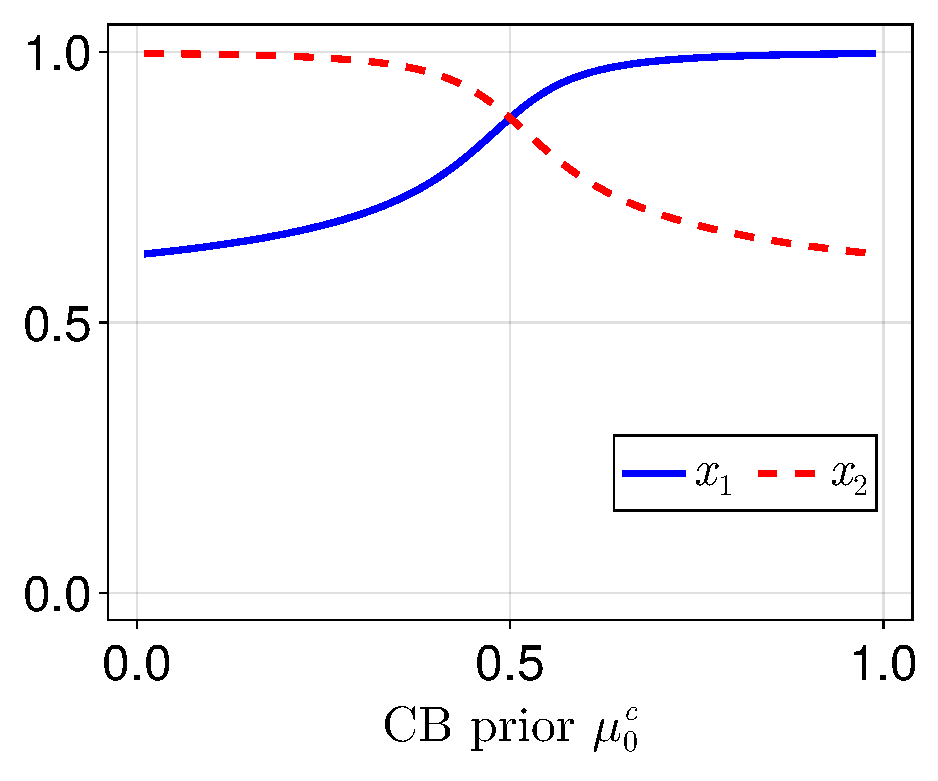
\includegraphics[width=0.49\textwidth]{figures/V8/γ_10/fig_optimal_π_across_μ_0_c_ω_1_1_ω_2_-1_δ_1.0_.pdf}
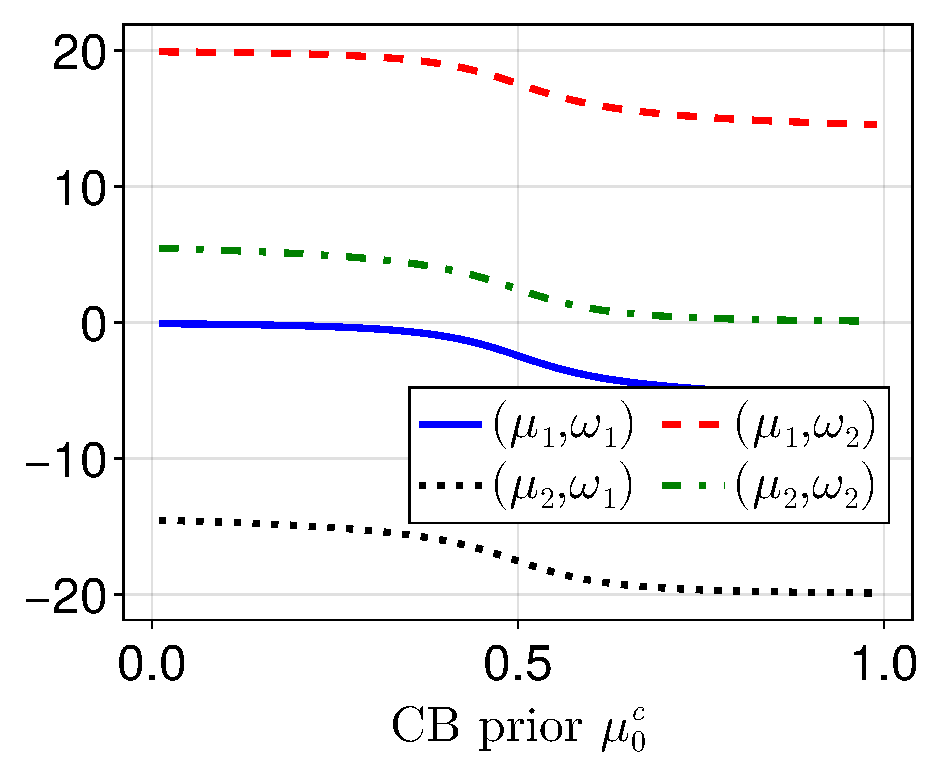
\includegraphics[width=0.49\textwidth]{figures/V8/γ_10/fig_posterior_across_μ_0_c_ω_1_1_ω_2_-1_δ_1.0_.pdf}
\caption{Comparative statics for $\mu_0^c$, when $\delta=1$, holding fixed all other parameters as in the benchmark.}
\label{FigureA4}
\end{figure}

\begin{figure}[H]
\centering
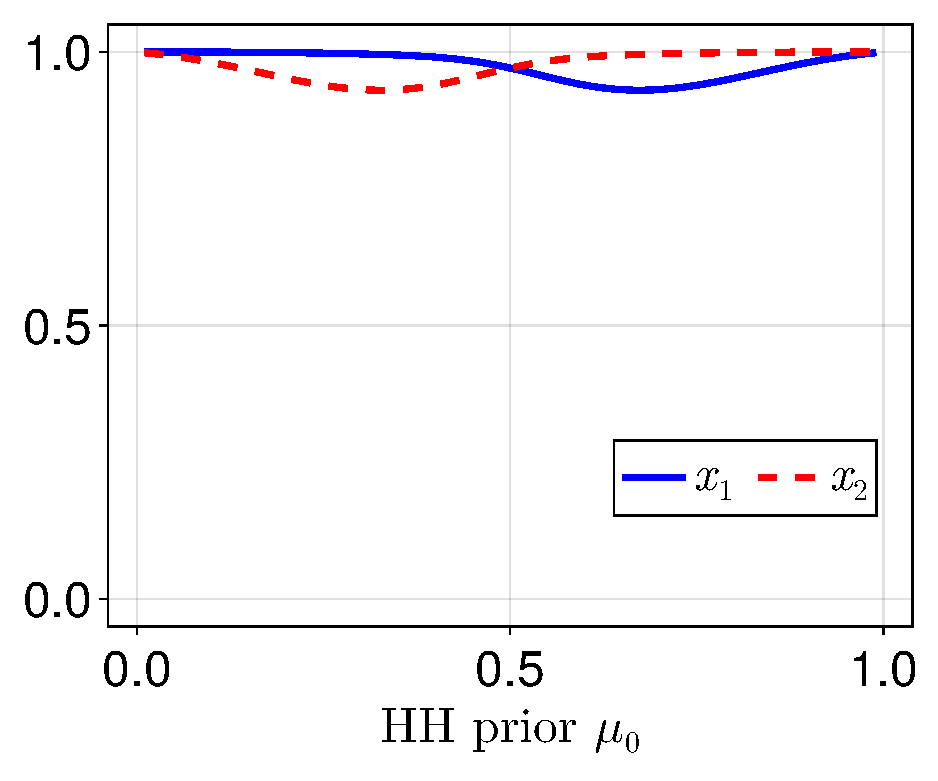
\includegraphics[width=0.49\textwidth]{figures/V8/γ_10/fig_optimal_π_across_μ_0_ω_1_2_ω_2_-2_δ_0.5_.pdf}
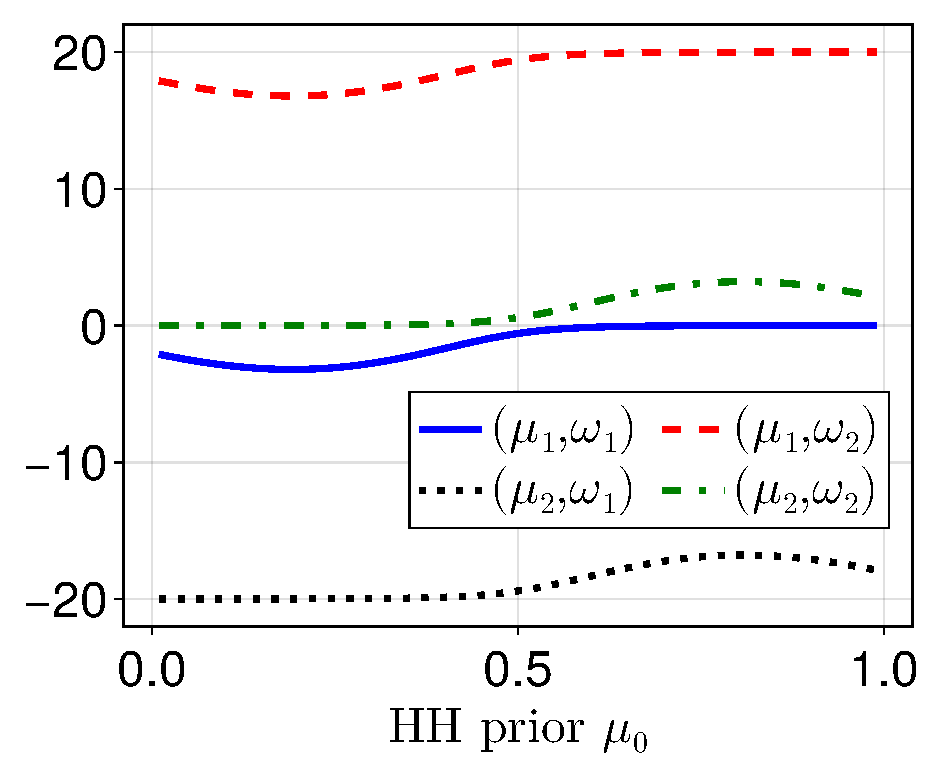
\includegraphics[width=0.49\textwidth]{figures/V8/γ_10/fig_posterior_across_μ_0_ω_1_2_ω_2_-2_δ_0.5_.pdf}
\caption{Comparative statics for $\mu_0$, when $(\omega_1,\omega_2)=(2,-2)$, holding fixed all other parameters as in the benchmark.}
\label{FigureA5}
\end{figure}

\begin{figure}[H]
\centering
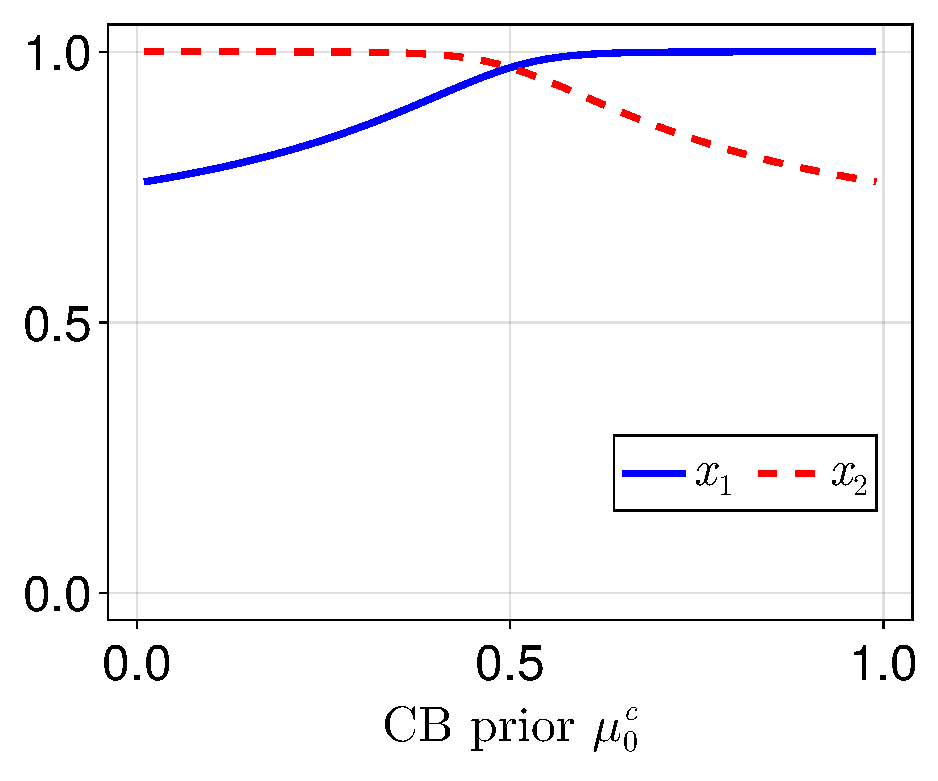
\includegraphics[width=0.49\textwidth]{figures/V8/γ_10/fig_optimal_π_across_μ_0_c_ω_1_2_ω_2_-2_δ_0.5_.pdf}
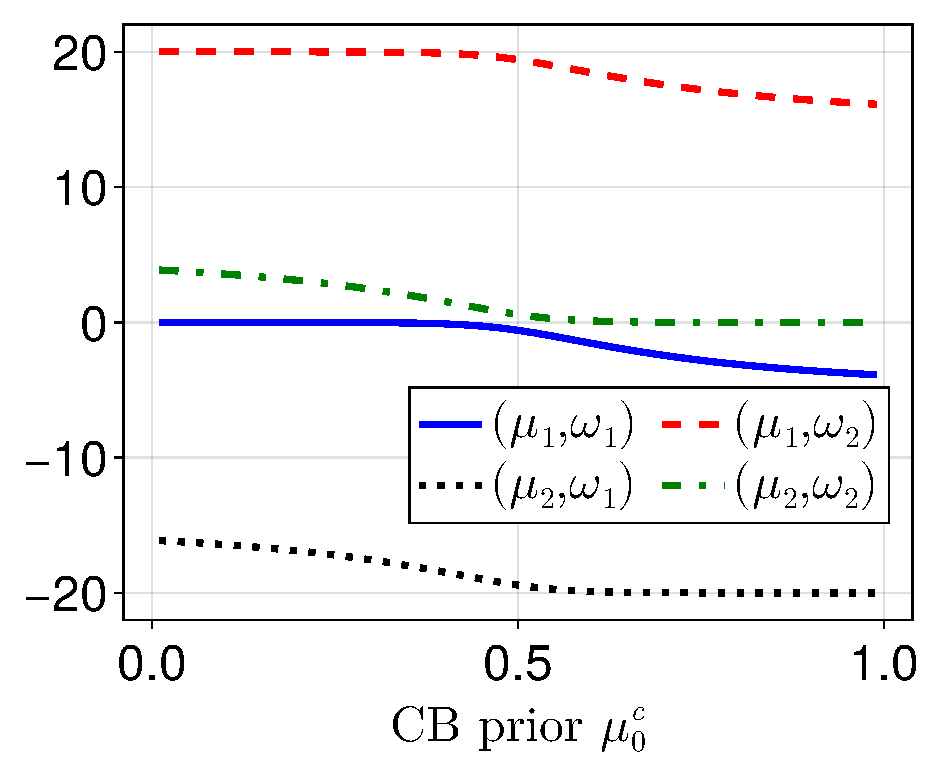
\includegraphics[width=0.49\textwidth]{figures/V8/γ_10/fig_posterior_across_μ_0_c_ω_1_2_ω_2_-2_δ_0.5_.pdf}
\caption{Comparative statics for $\mu_0^c$, when $(\omega_1,\omega_2)=(2,-2)$, holding fixed all other parameters as in the benchmark.}
\label{FigureA6}
\end{figure}

\begin{figure}[H]
\centering
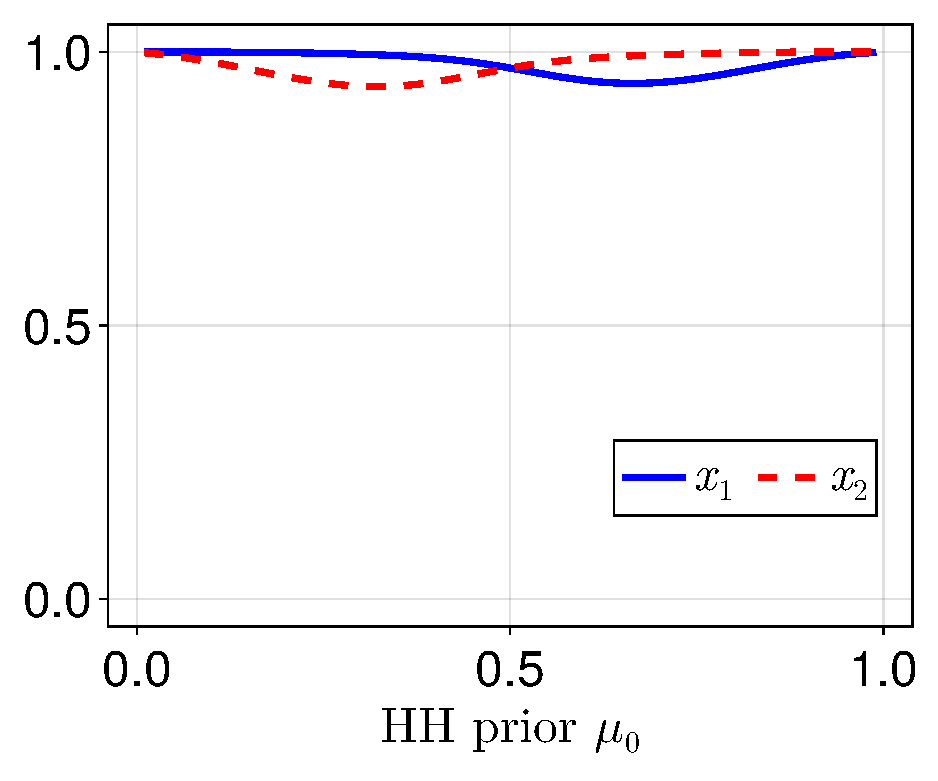
\includegraphics[width=0.49\textwidth]{figures/V8/γ_10/fig_optimal_π_across_μ_0_ω_1_2_ω_2_-1_δ_0.5_.pdf}
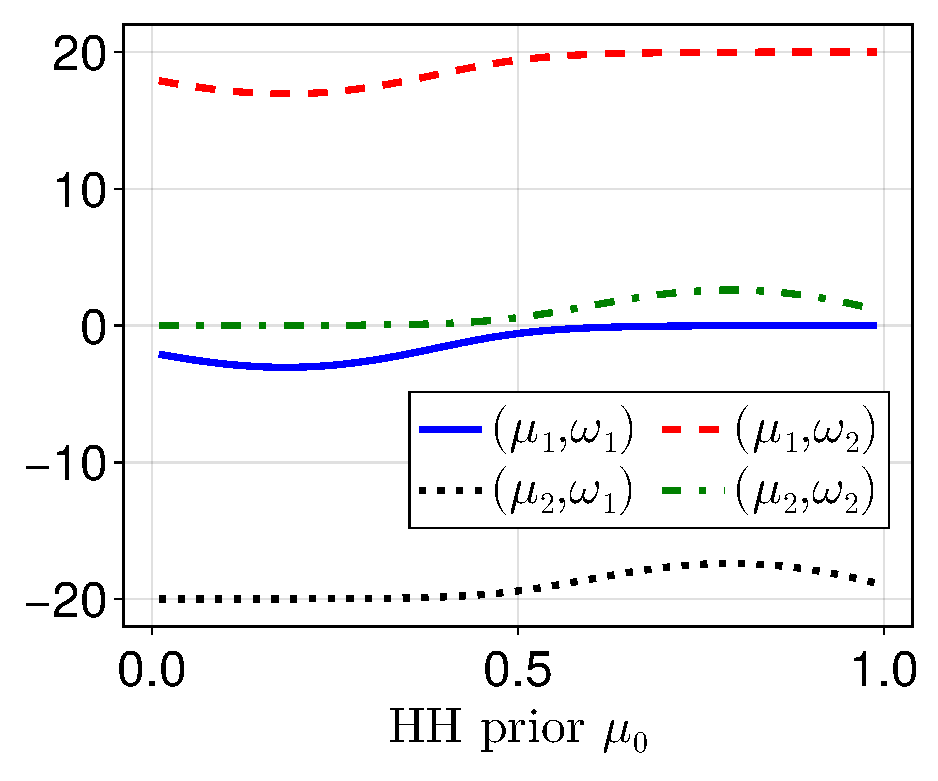
\includegraphics[width=0.49\textwidth]{figures/V8/γ_10/fig_posterior_across_μ_0_ω_1_2_ω_2_-1_δ_0.5_.pdf}
\caption{Comparative statics for $\mu_0$, when $(\omega_1,\omega_2)=(2,-1)$, holding fixed all other parameters as in the benchmark.}
\label{FigureA7}
\end{figure}

\begin{figure}[H]
\centering
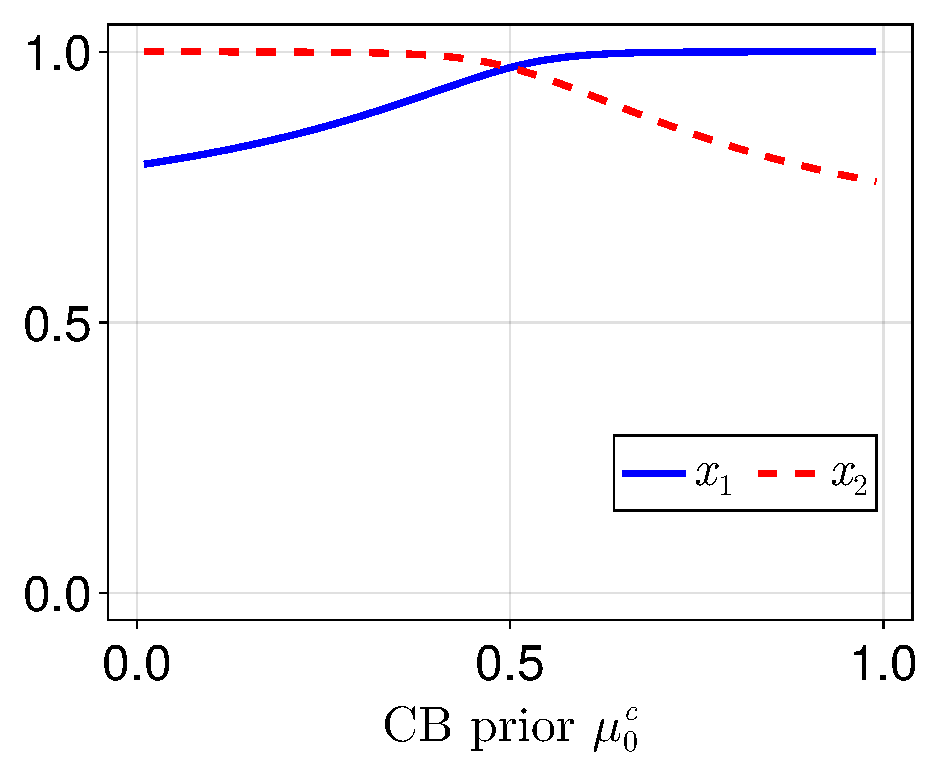
\includegraphics[width=0.49\textwidth]{figures/V8/γ_10/fig_optimal_π_across_μ_0_c_ω_1_2_ω_2_-1_δ_0.5_.pdf}
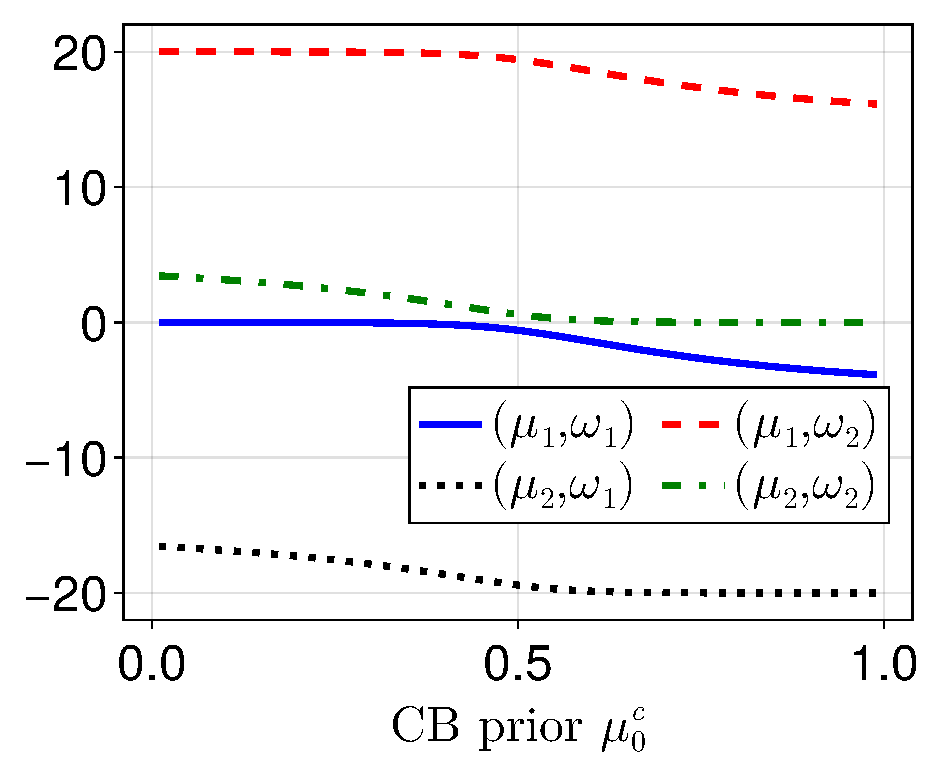
\includegraphics[width=0.49\textwidth]{figures/V8/γ_10/fig_posterior_across_μ_0_c_ω_1_2_ω_2_-1_δ_0.5_.pdf}
\caption{Comparative statics for $\mu_0^c$, when $(\omega_1,\omega_2)=(2,-1)$, holding fixed all other parameters as in the benchmark.}
\label{FigureA8}
\end{figure}

\begin{figure}[H]
\centering
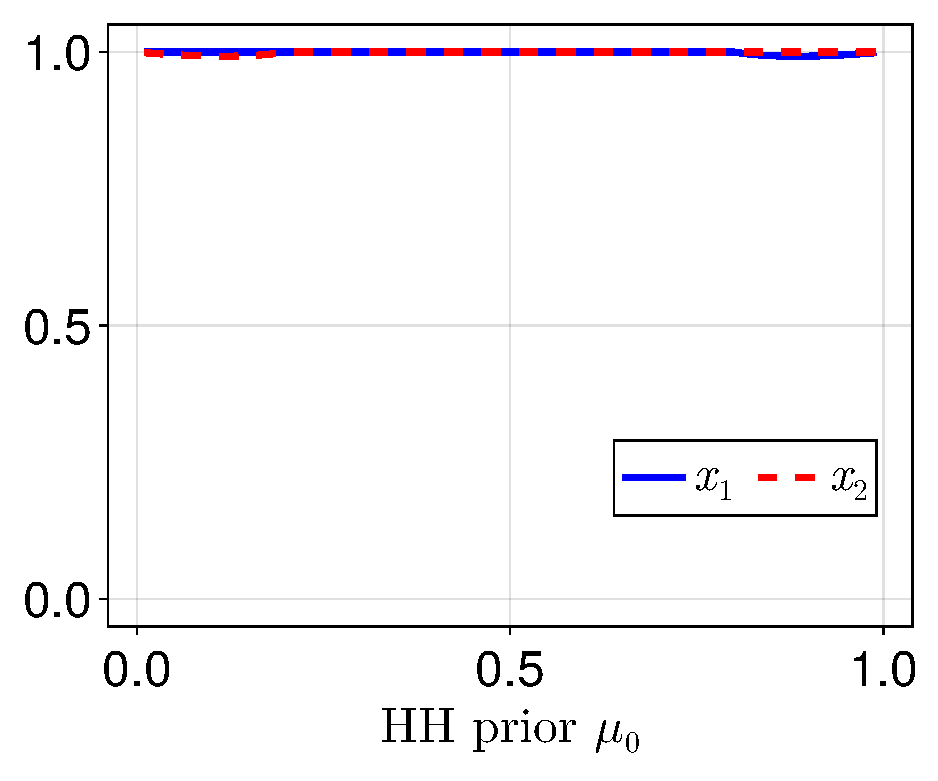
\includegraphics[width=0.49\textwidth]{figures/V8/γ_10/fig_optimal_π_across_μ_0_ω_1_2_ω_2_-2_δ_0.0_.pdf}
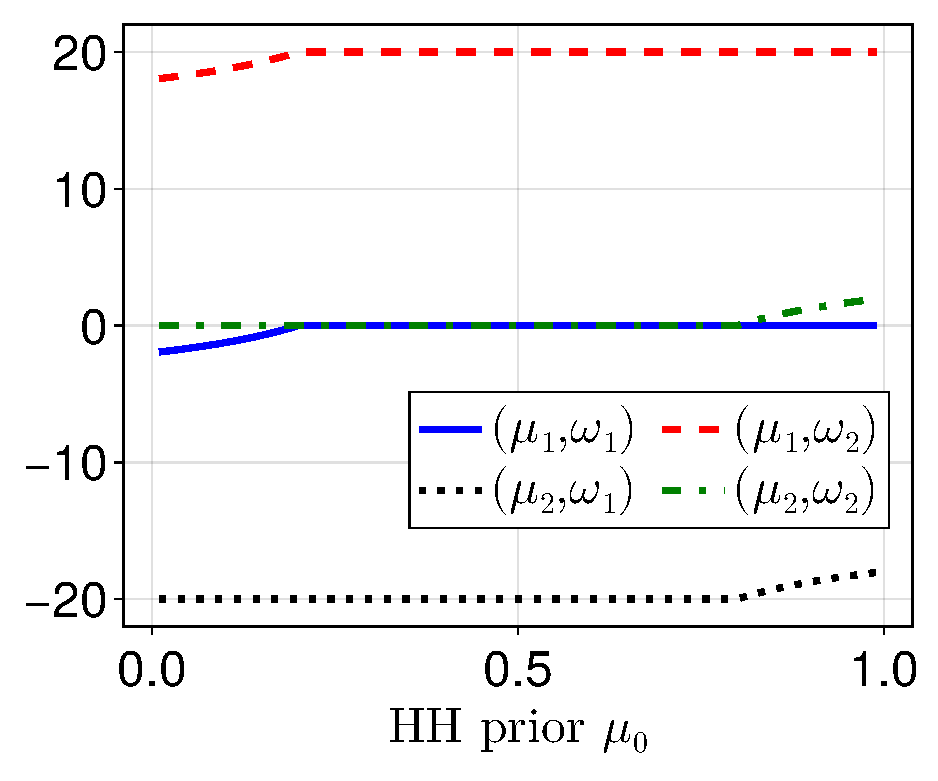
\includegraphics[width=0.49\textwidth]{figures/V8/γ_10/fig_posterior_across_μ_0_ω_1_2_ω_2_-2_δ_0.0_.pdf}
\caption{Comparative statics for $\mu_0$, when $(\delta,\omega_1,\omega_2)=(0,2,-2)$, holding fixed all other parameters as in the benchmark.}
\label{FigureA9}
\end{figure}

\begin{figure}[H]
\centering
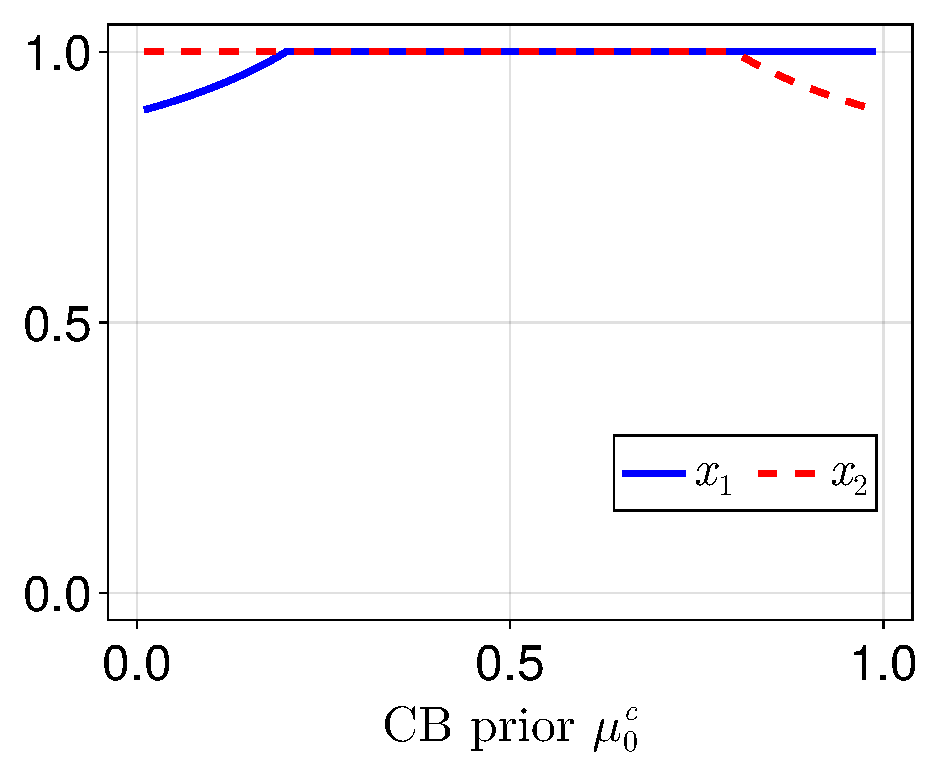
\includegraphics[width=0.49\textwidth]{figures/V8/γ_10/fig_optimal_π_across_μ_0_c_ω_1_2_ω_2_-2_δ_0.0_.pdf}
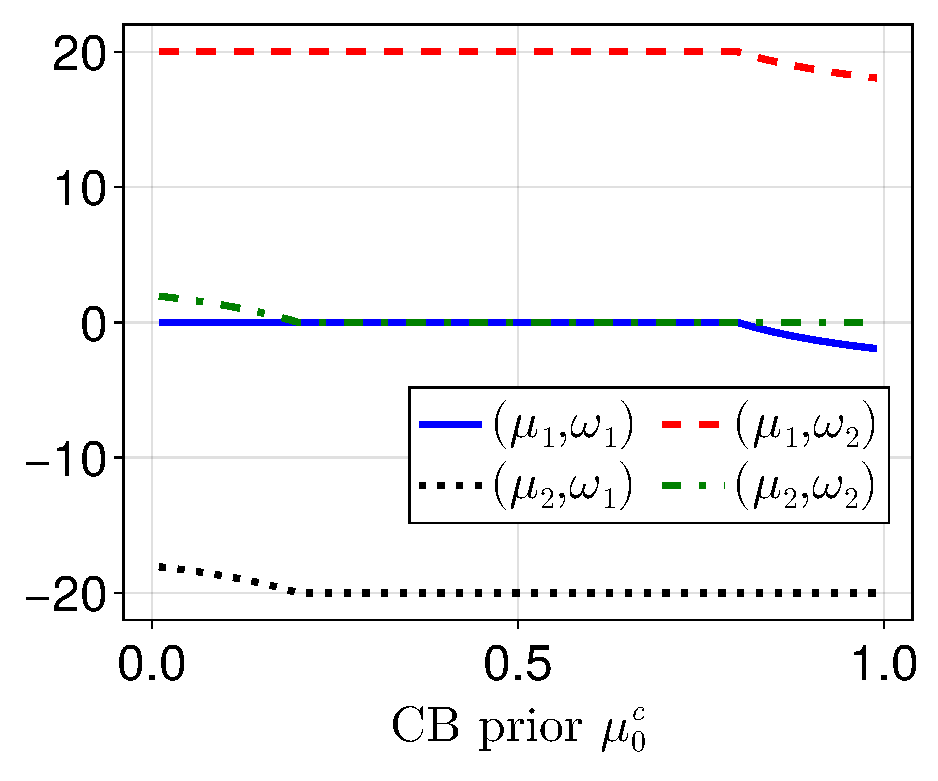
\includegraphics[width=0.49\textwidth]{figures/V8/γ_10/fig_posterior_across_μ_0_c_ω_1_2_ω_2_-2_δ_0.0_.pdf}
\caption{Comparative statics for $\mu_0^c$, when $(\delta,\omega_1,\omega_2)=(0,2,-2)$, holding fixed all other parameters as in the benchmark.}
\label{FigureA10}
\end{figure}

\begin{figure}[H]
\centering
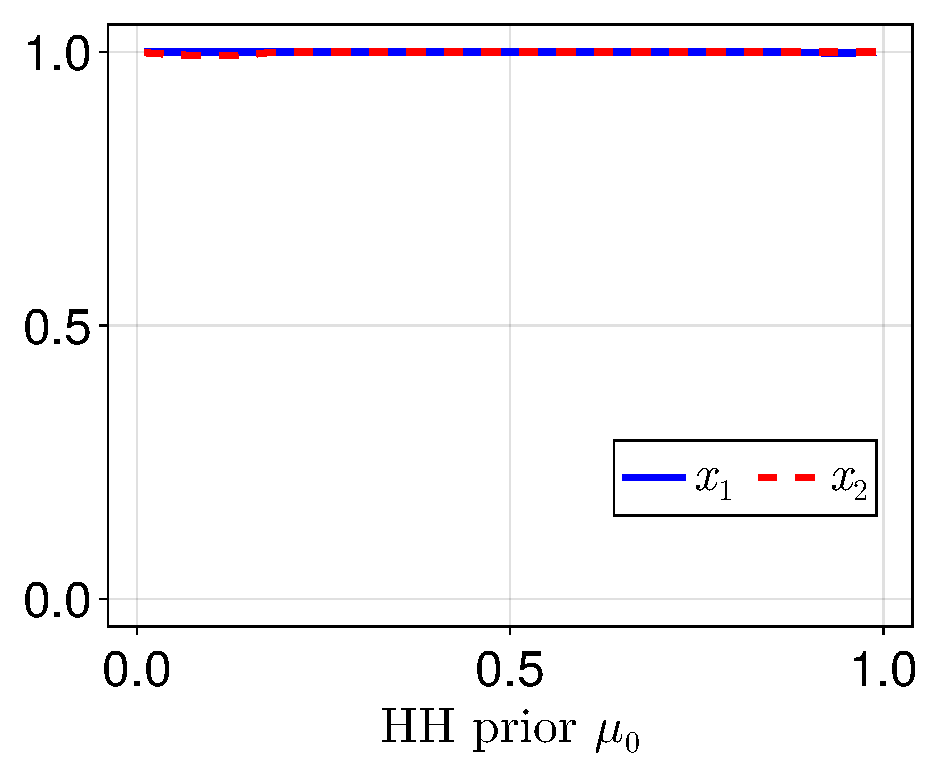
\includegraphics[width=0.49\textwidth]{figures/V8/γ_10/fig_optimal_π_across_μ_0_ω_1_2_ω_2_-1_δ_0.0_.pdf}
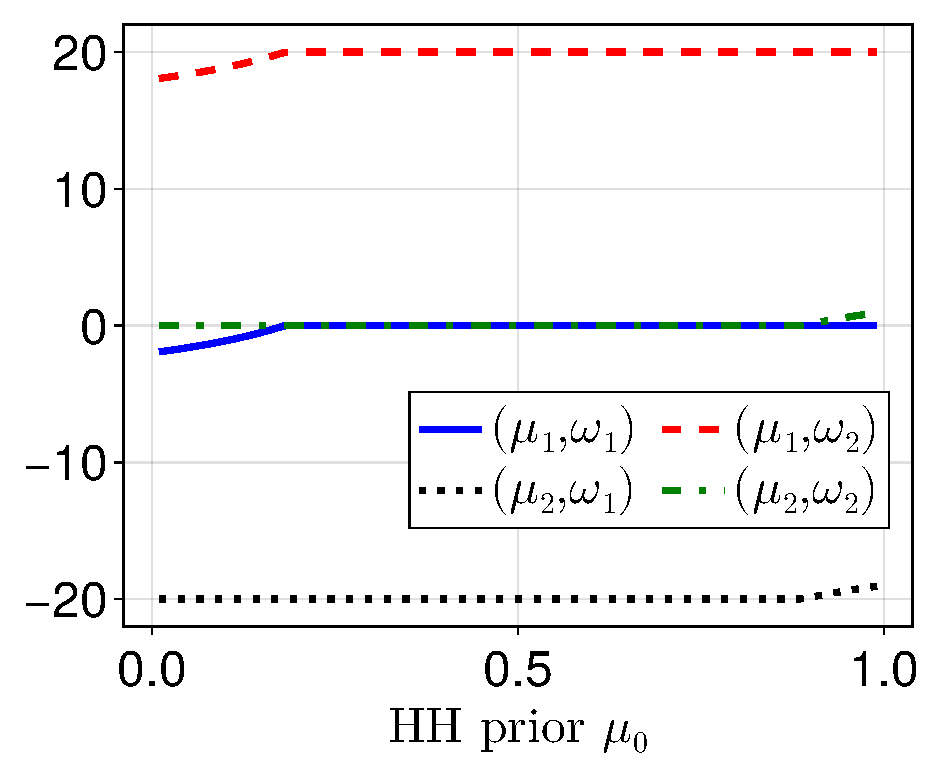
\includegraphics[width=0.49\textwidth]{figures/V8/γ_10/fig_posterior_across_μ_0_ω_1_2_ω_2_-1_δ_0.0_.pdf}
\caption{Comparative statics for $\mu_0$, when $(\delta,\omega_1,\omega_2)=(0,2,-1)$, holding fixed all other parameters as in the benchmark.}
\label{FigureA11}
\end{figure}

\begin{figure}[H]
\centering
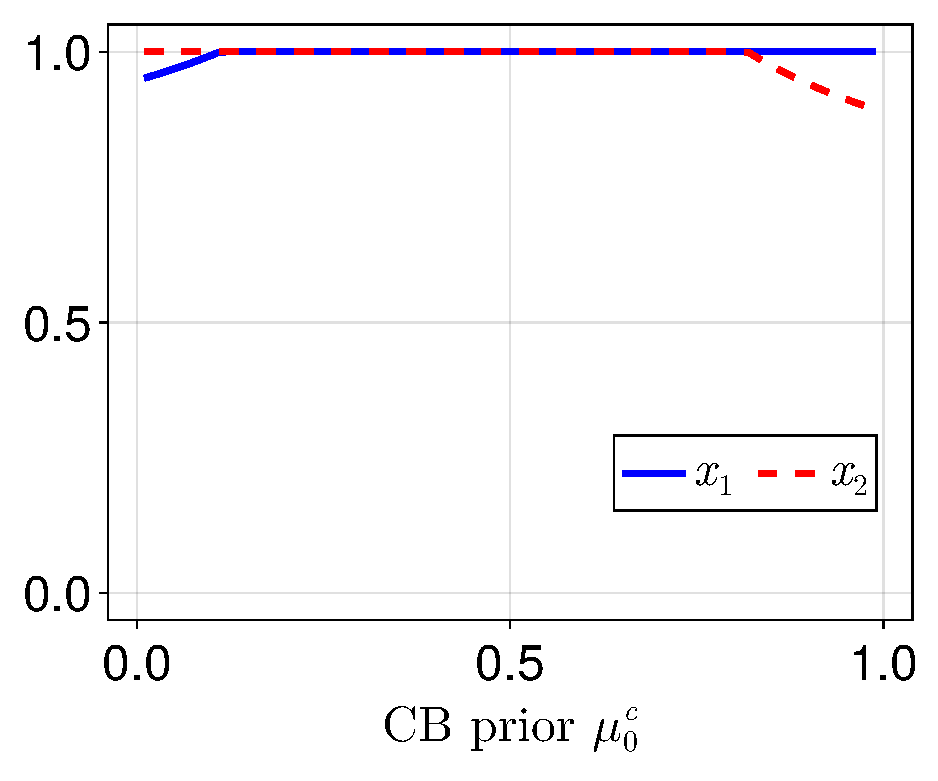
\includegraphics[width=0.49\textwidth]{figures/V8/γ_10/fig_optimal_π_across_μ_0_c_ω_1_2_ω_2_-1_δ_0.0_.pdf}
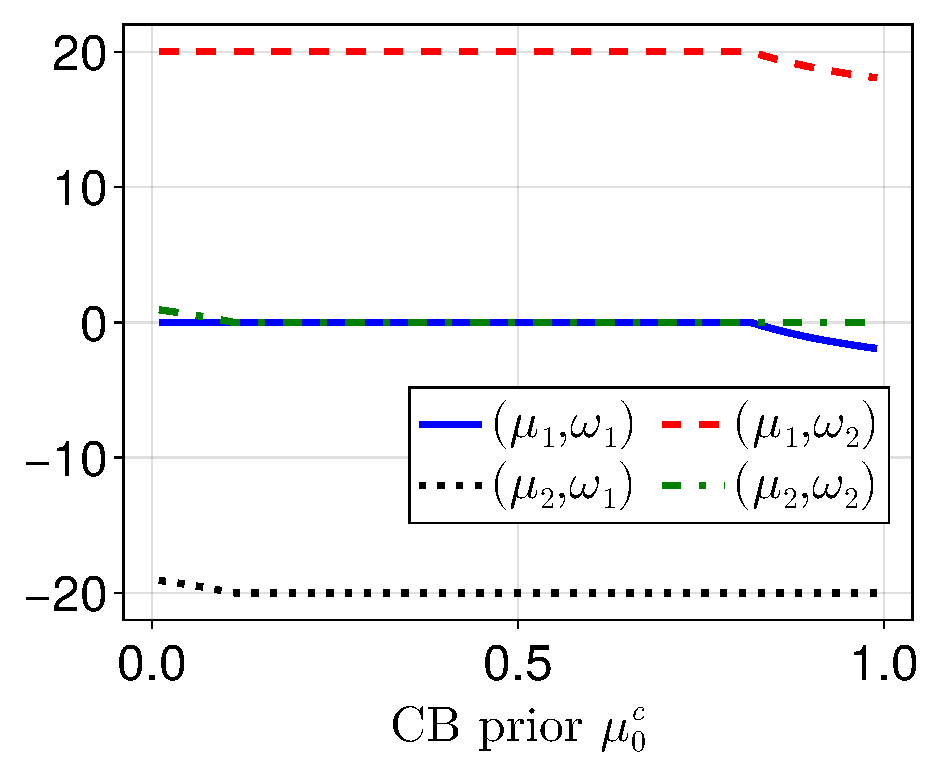
\includegraphics[width=0.49\textwidth]{figures/V8/γ_10/fig_posterior_across_μ_0_c_ω_1_2_ω_2_-1_δ_0.0_.pdf}
\caption{Comparative statics for $\mu_0^c$, when $(\delta,\omega_1,\omega_2)=(0,2,-1)$, holding fixed all other parameters as in the benchmark.}
\label{FigureA12}
\end{figure}

Third, $(\delta,\omega_1,\omega_2)=(1,2,-2)$.

\begin{figure}[H]
\centering
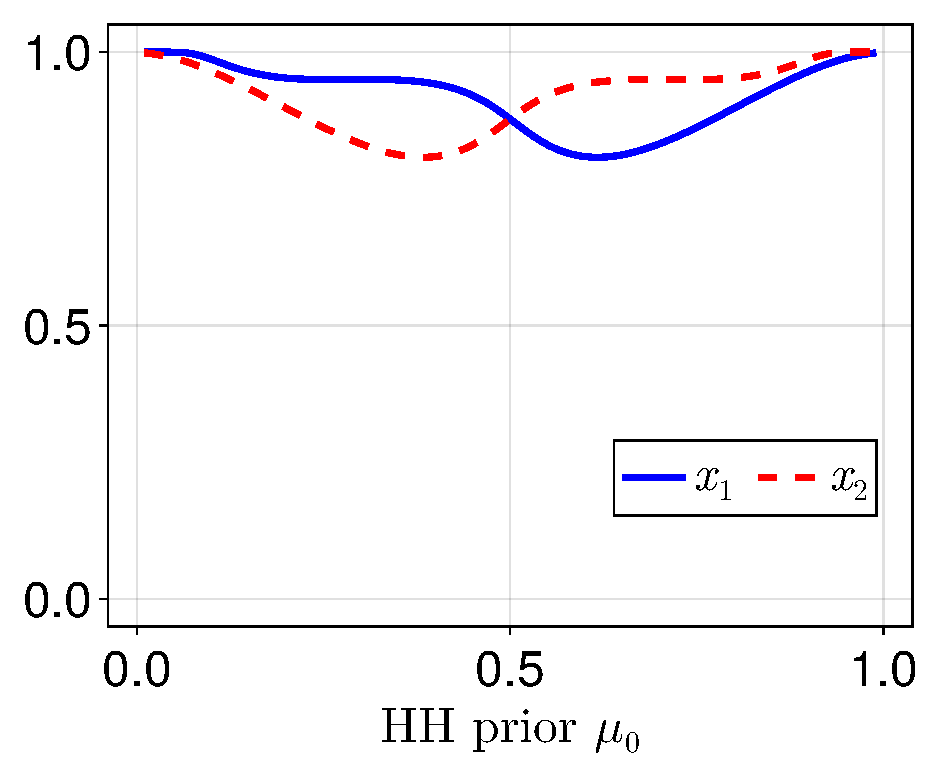
\includegraphics[width=0.49\textwidth]{figures/V8/γ_10/fig_optimal_π_across_μ_0_ω_1_2_ω_2_-2_δ_1.0_.pdf}
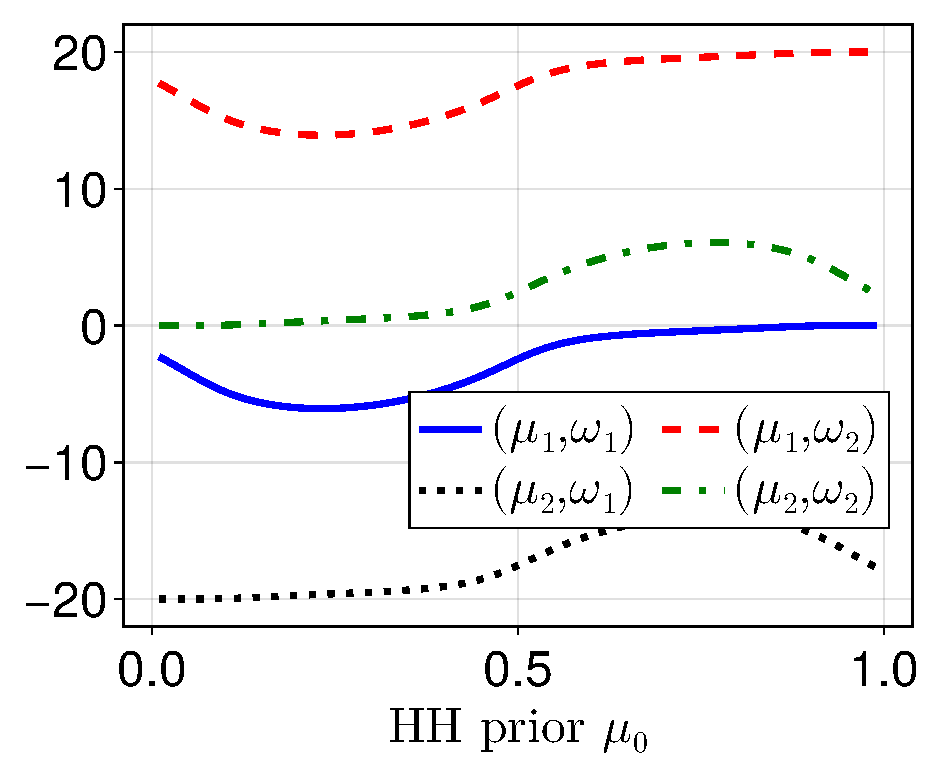
\includegraphics[width=0.49\textwidth]{figures/V8/γ_10/fig_posterior_across_μ_0_ω_1_2_ω_2_-2_δ_1.0_.pdf}
\caption{Comparative statics for $\mu_0$, when $(\delta,\omega_1,\omega_2)=(1,2,-2)$, holding fixed all other parameters as in the benchmark.}
\label{FigureA13}
\end{figure}

\begin{figure}[H]
\centering
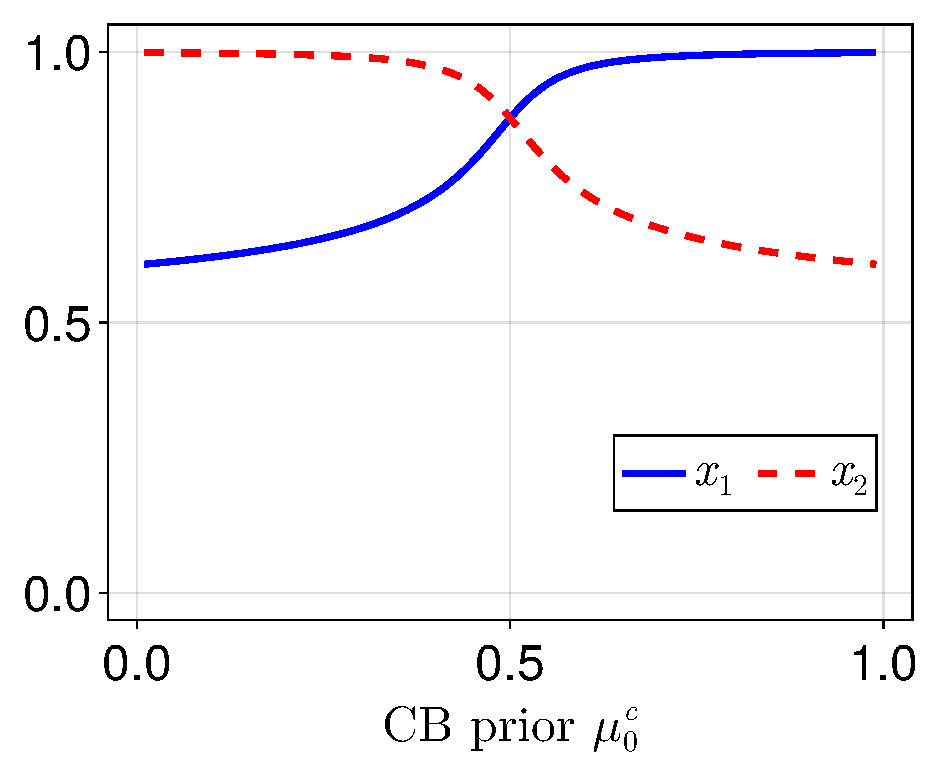
\includegraphics[width=0.49\textwidth]{figures/V8/γ_10/fig_optimal_π_across_μ_0_c_ω_1_2_ω_2_-2_δ_1.0_.pdf}
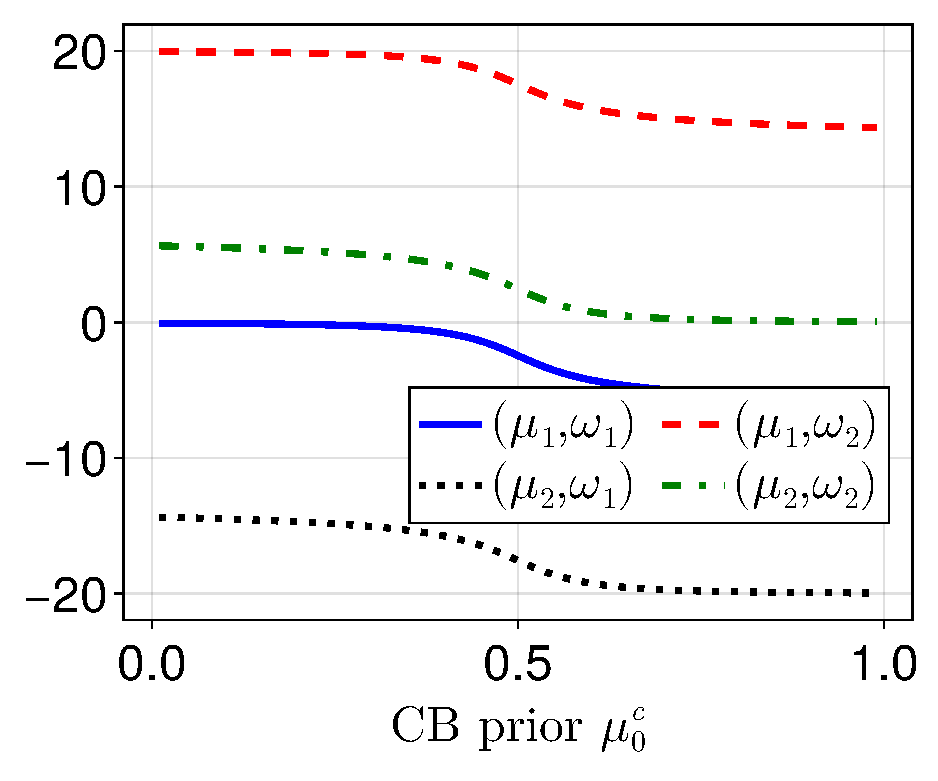
\includegraphics[width=0.49\textwidth]{figures/V8/γ_10/fig_posterior_across_μ_0_c_ω_1_2_ω_2_-2_δ_1.0_.pdf}
\caption{Comparative statics for $\mu_0^c$, when $(\delta,\omega_1,\omega_2)=(1,2,-2)$, holding fixed all other parameters as in the benchmark.}
\label{FigureA14}
\end{figure}

\begin{figure}[H]
\centering
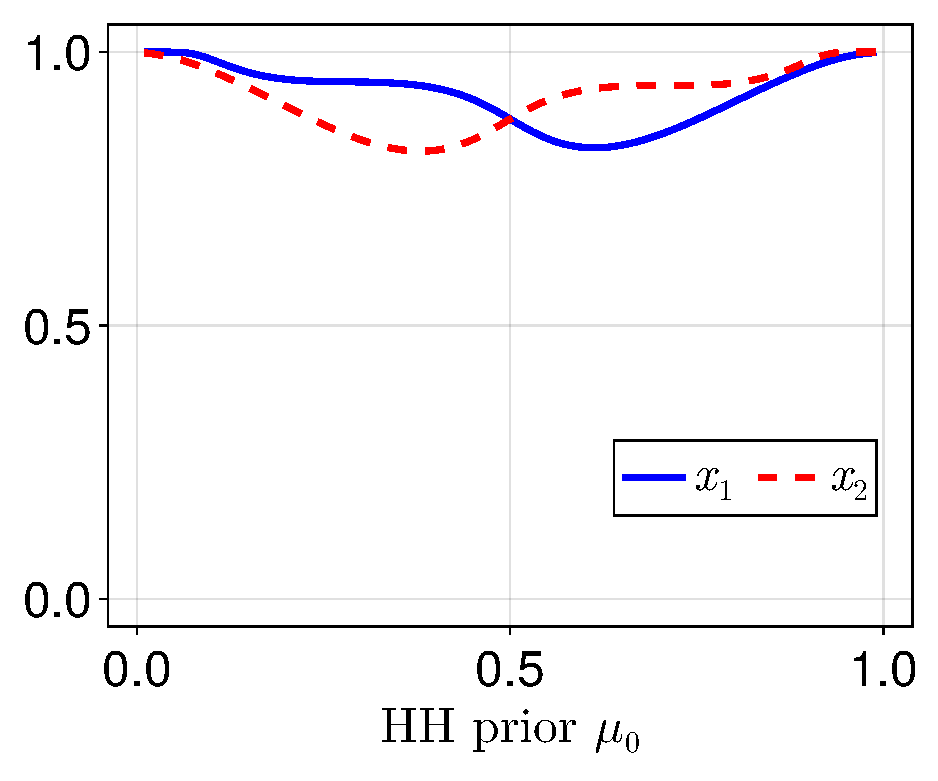
\includegraphics[width=0.49\textwidth]{figures/V8/γ_10/fig_optimal_π_across_μ_0_ω_1_2_ω_2_-1_δ_1.0_.pdf}
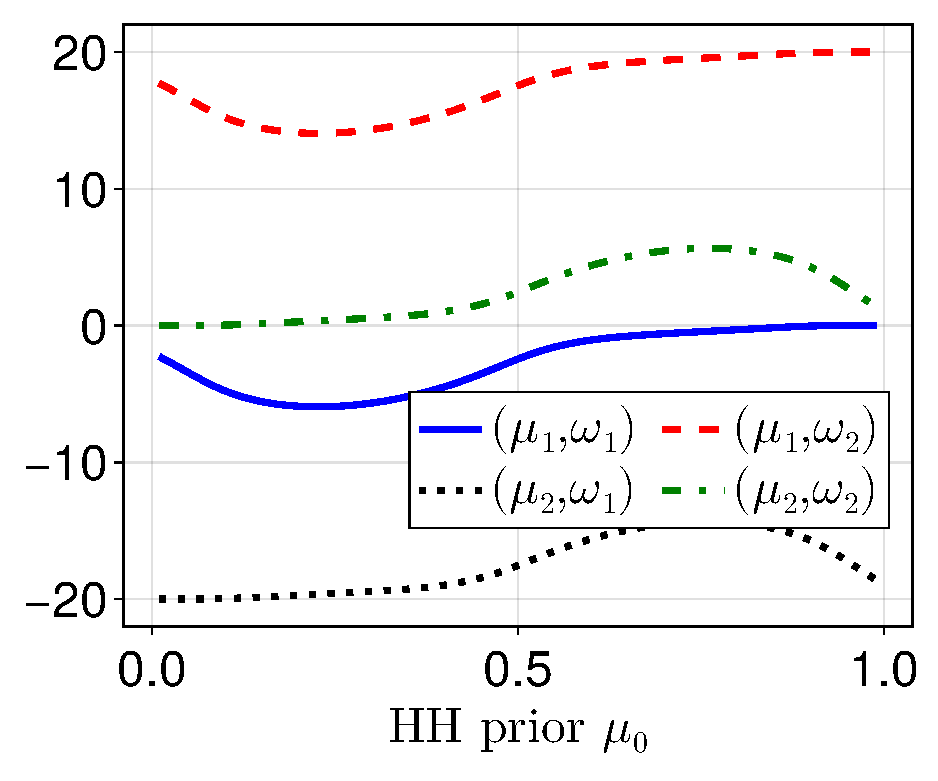
\includegraphics[width=0.49\textwidth]{figures/V8/γ_10/fig_posterior_across_μ_0_ω_1_2_ω_2_-1_δ_1.0_.pdf}
\caption{Comparative statics for $\mu_0$, when $(\delta,\omega_1,\omega_2)=(1,2,-1)$, holding fixed all other parameters as in the benchmark.}
\label{FigureA15}
\end{figure}

\begin{figure}[H]
\centering
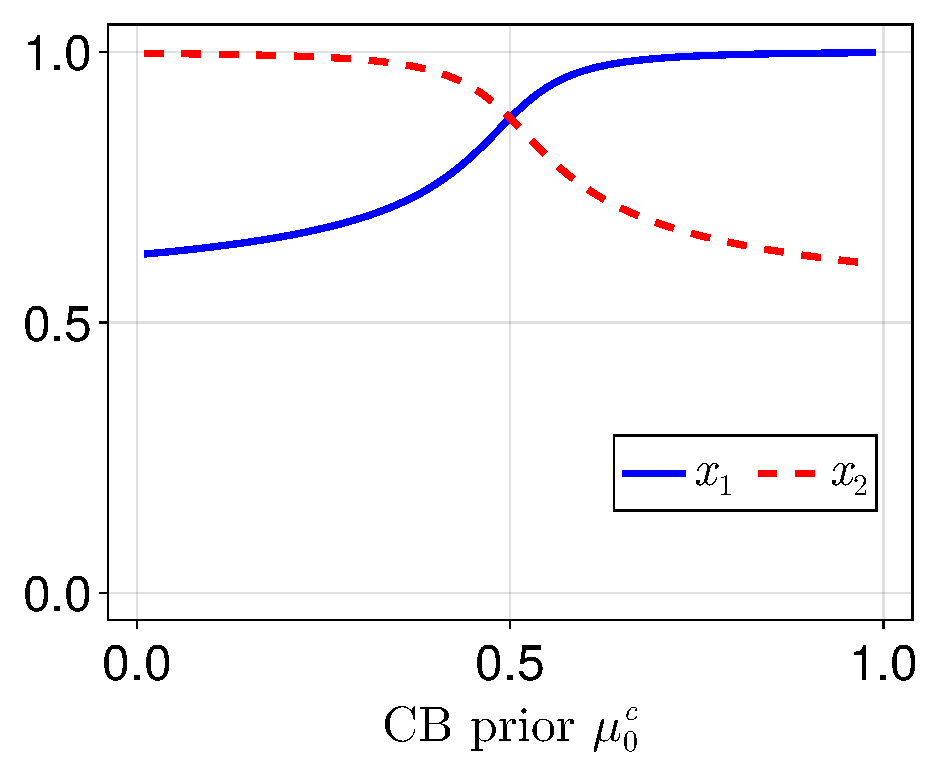
\includegraphics[width=0.49\textwidth]{figures/V8/γ_10/fig_optimal_π_across_μ_0_c_ω_1_2_ω_2_-1_δ_1.0_.pdf}
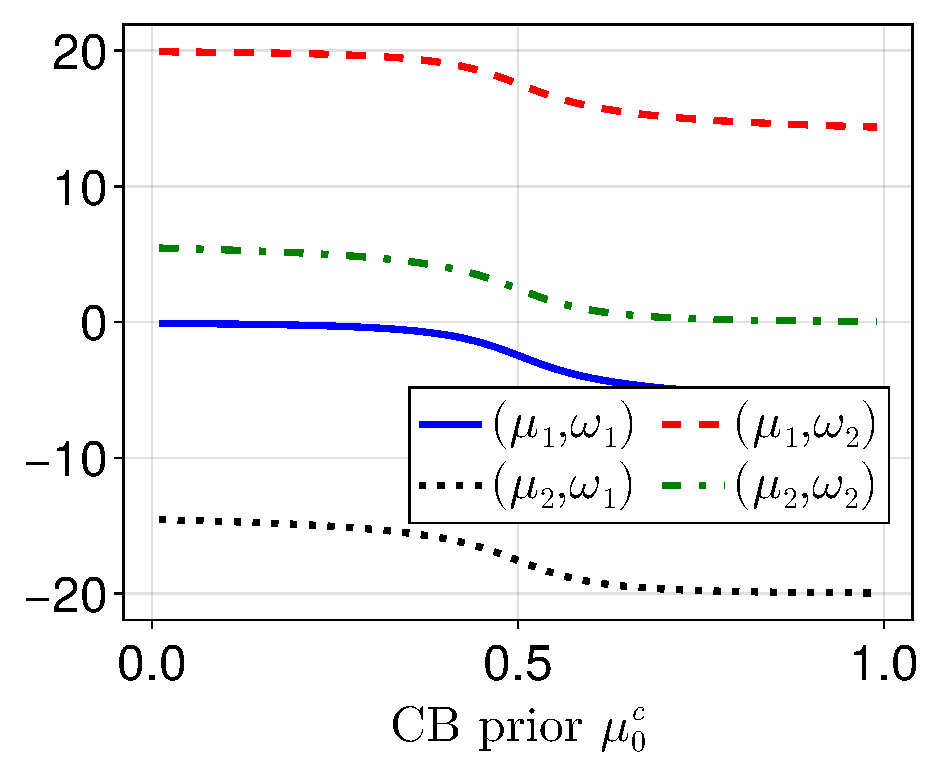
\includegraphics[width=0.49\textwidth]{figures/V8/γ_10/fig_posterior_across_μ_0_c_ω_1_2_ω_2_-1_δ_1.0_.pdf}
\caption{Comparative statics for $\mu_0^c$, when $(\delta,\omega_1,\omega_2)=(1,2,-1)$, holding fixed all other parameters as in the benchmark.}
\label{FigureA16}
\end{figure}

\begin{figure}[H]
\centering
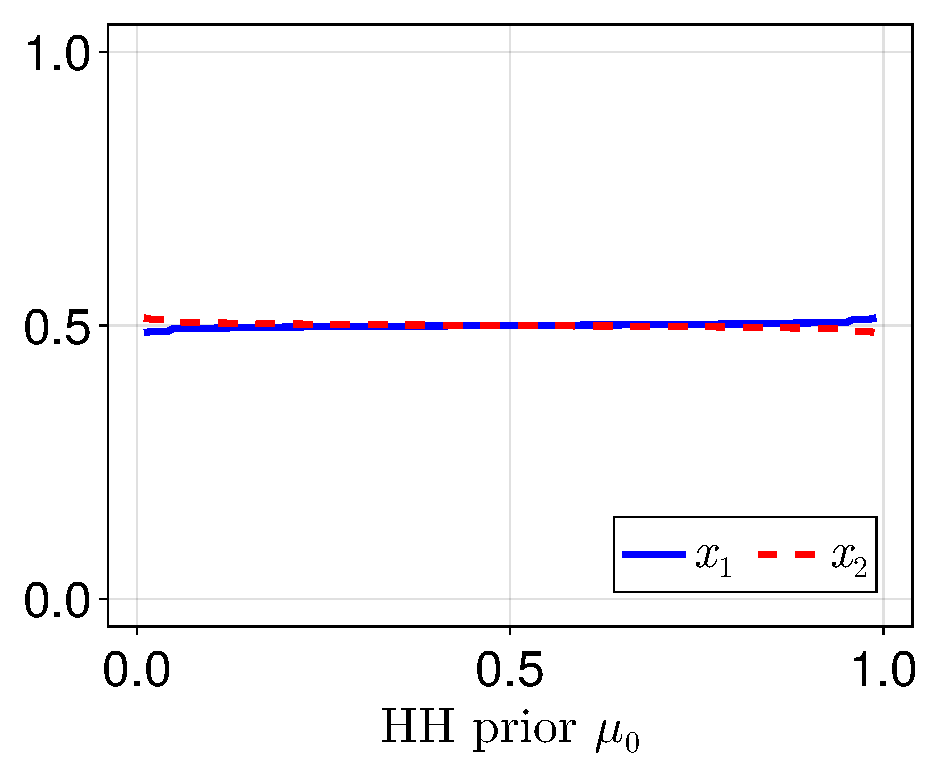
\includegraphics[width=0.49\textwidth]{figures/V8/γ_1/fig_optimal_π_across_μ_0_ω_1_2_ω_2_-2_δ_0.5_.pdf}
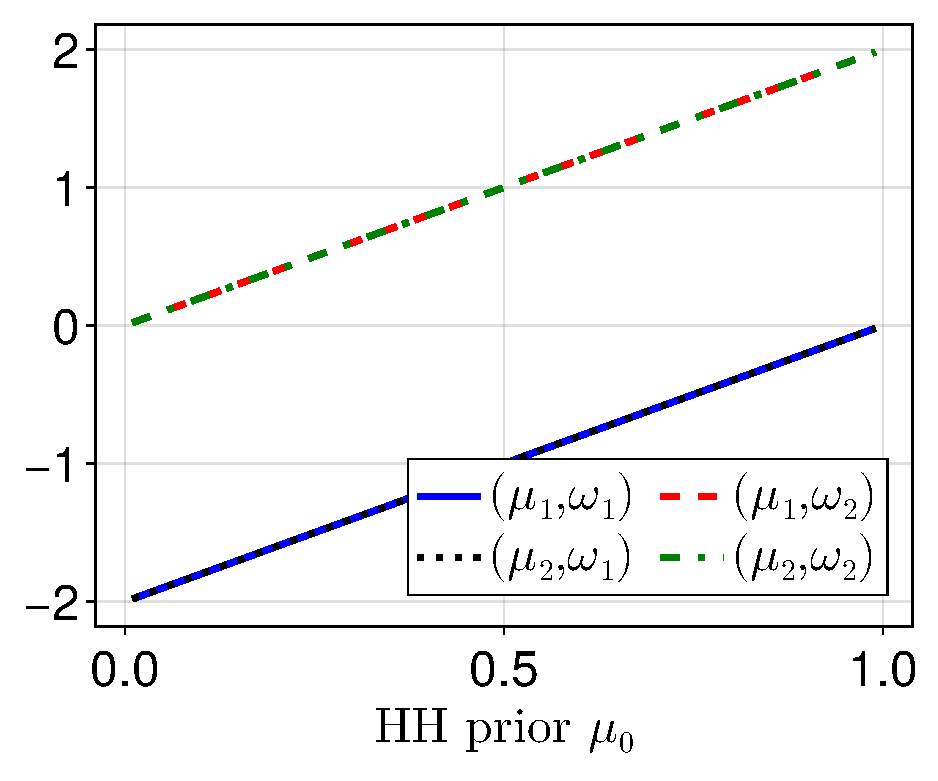
\includegraphics[width=0.49\textwidth]{figures/V8/γ_1/fig_posterior_across_μ_0_ω_1_2_ω_2_-2_δ_0.5_.pdf}
\caption{Comparative statics for $\mu_0$, when $(\omega_1,\omega_2)=(2,-2)$, holding fixed all other parameters as in the benchmark.}
\label{FigureA17}
\end{figure}

\begin{figure}[H]
\centering
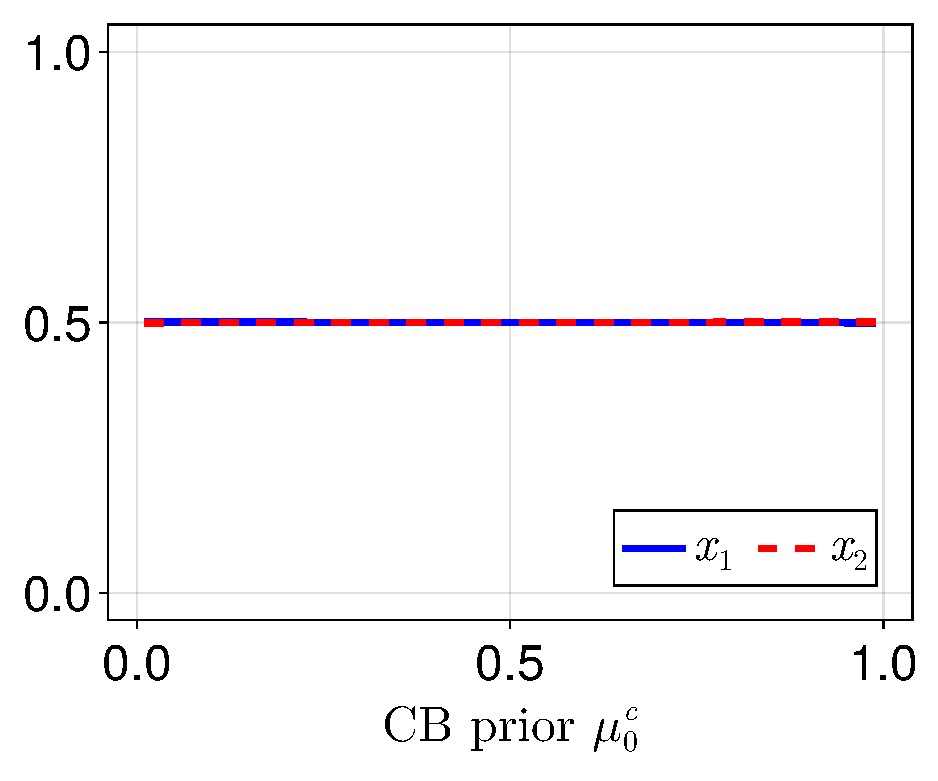
\includegraphics[width=0.49\textwidth]{figures/V8/γ_1/fig_optimal_π_across_μ_0_c_ω_1_2_ω_2_-2_δ_0.5_.pdf}
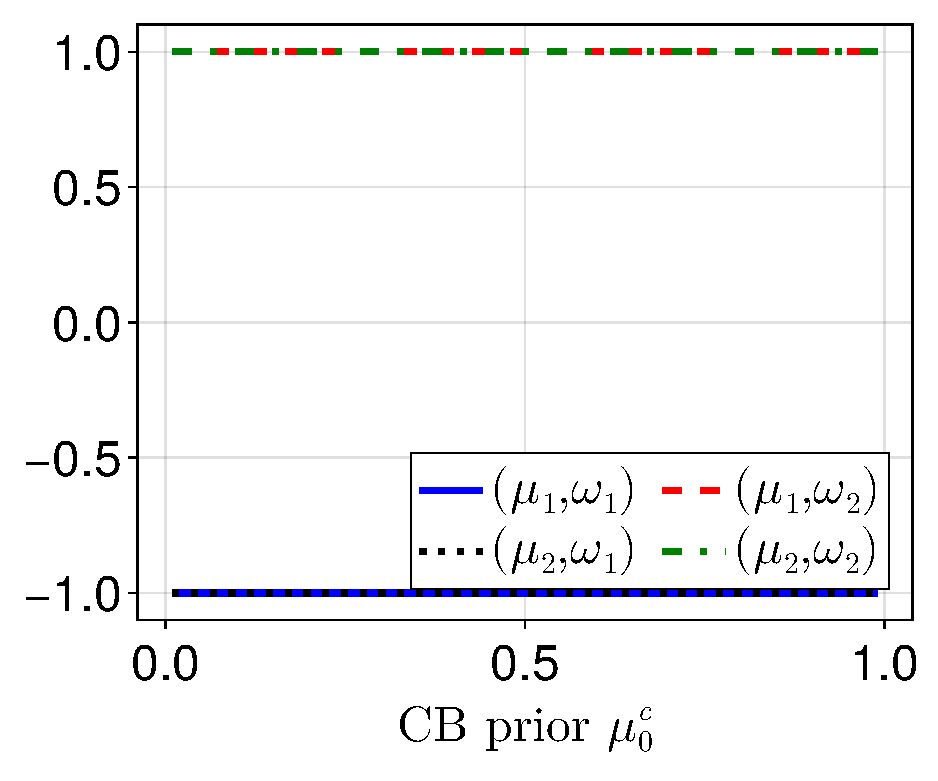
\includegraphics[width=0.49\textwidth]{figures/V8/γ_1/fig_posterior_across_μ_0_c_ω_1_2_ω_2_-2_δ_0.5_.pdf}
\caption{Comparative statics for $\mu_0^c$, when $(\omega_1,\omega_2)=(2,-2)$, holding fixed all other parameters as in the benchmark.}
\label{FigureA18}
\end{figure}

\begin{figure}[H]
\centering
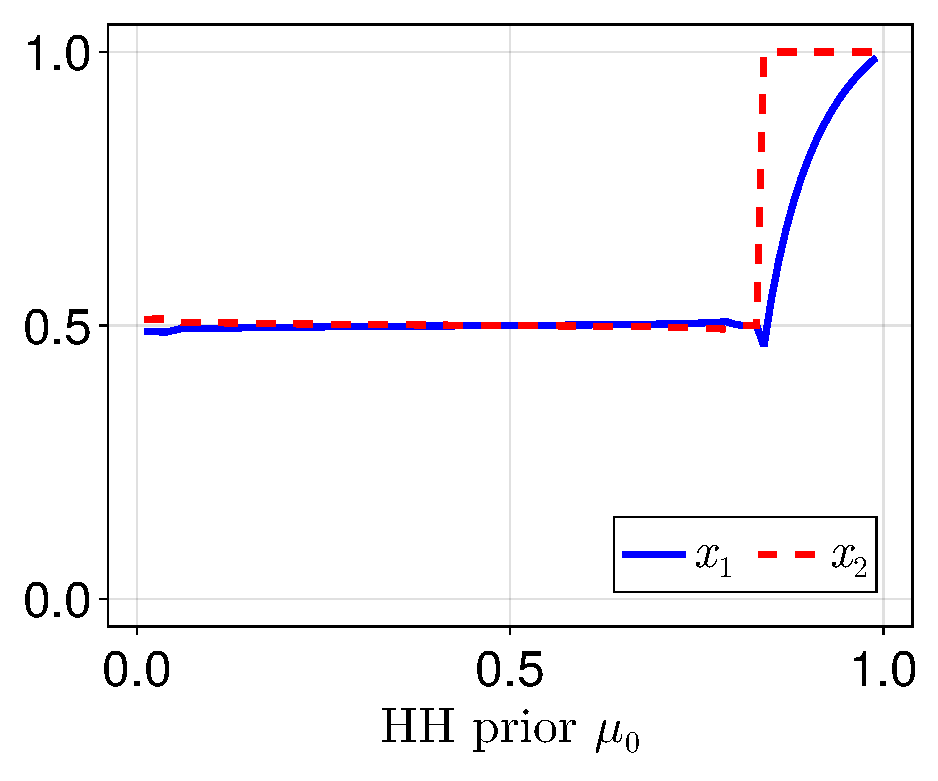
\includegraphics[width=0.49\textwidth]{figures/V8/γ_1/fig_optimal_π_across_μ_0_ω_1_2_ω_2_-1_δ_0.5_.pdf}
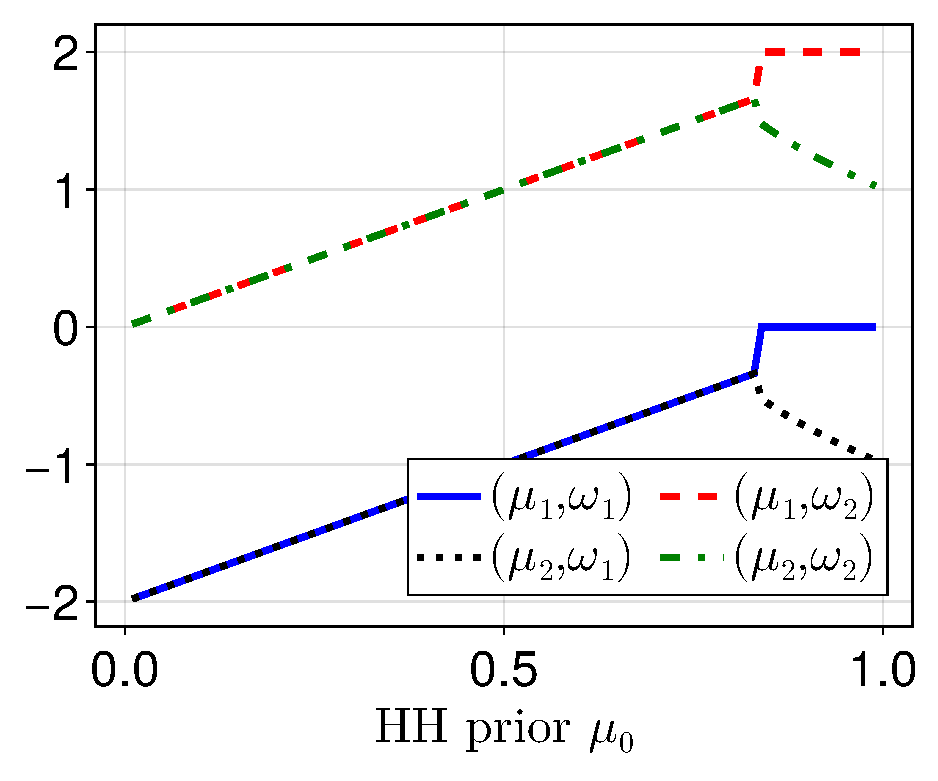
\includegraphics[width=0.49\textwidth]{figures/V8/γ_1/fig_posterior_across_μ_0_ω_1_2_ω_2_-1_δ_0.5_.pdf}
\caption{Comparative statics for $\mu_0$, when $(\omega_1,\omega_2)=(2,-1)$, holding fixed all other parameters as in the benchmark.}
\label{FigureA19}
\end{figure}

\begin{figure}[H]
\centering
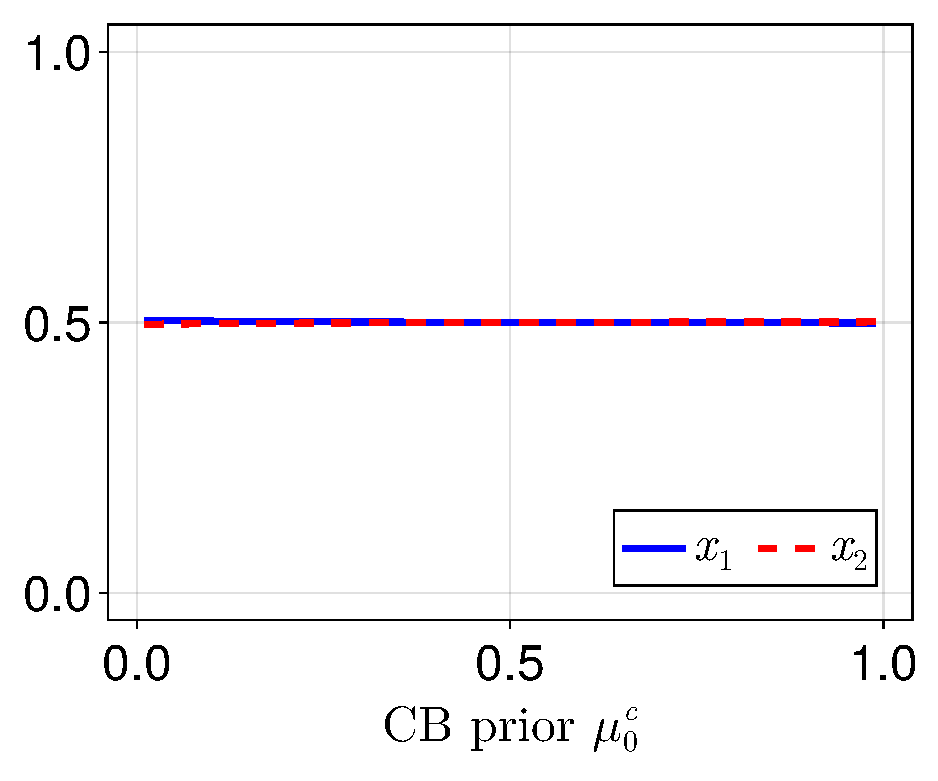
\includegraphics[width=0.49\textwidth]{figures/V8/γ_1/fig_optimal_π_across_μ_0_c_ω_1_2_ω_2_-1_δ_0.5_.pdf}
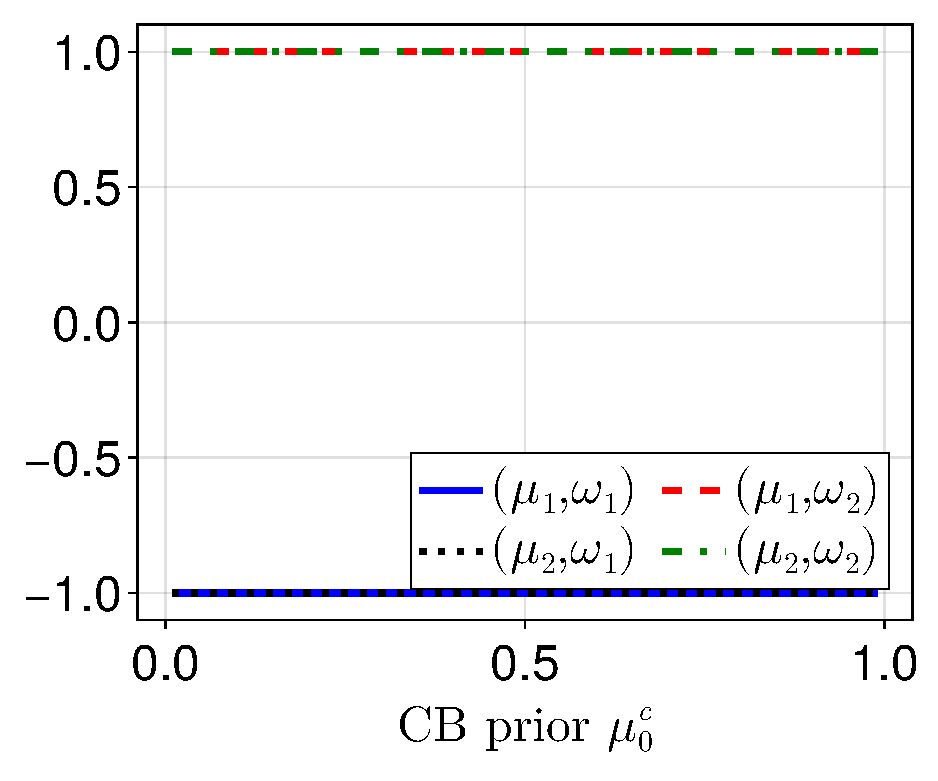
\includegraphics[width=0.49\textwidth]{figures/V8/γ_1/fig_posterior_across_μ_0_c_ω_1_2_ω_2_-1_δ_0.5_.pdf}
\caption{Comparative statics for $\mu_0^c$, when $(\omega_1,\omega_2)=(2,-1)$, holding fixed all other parameters as in the benchmark.}
\label{FigureA20}
\end{figure}

\begin{figure}[H]
\centering
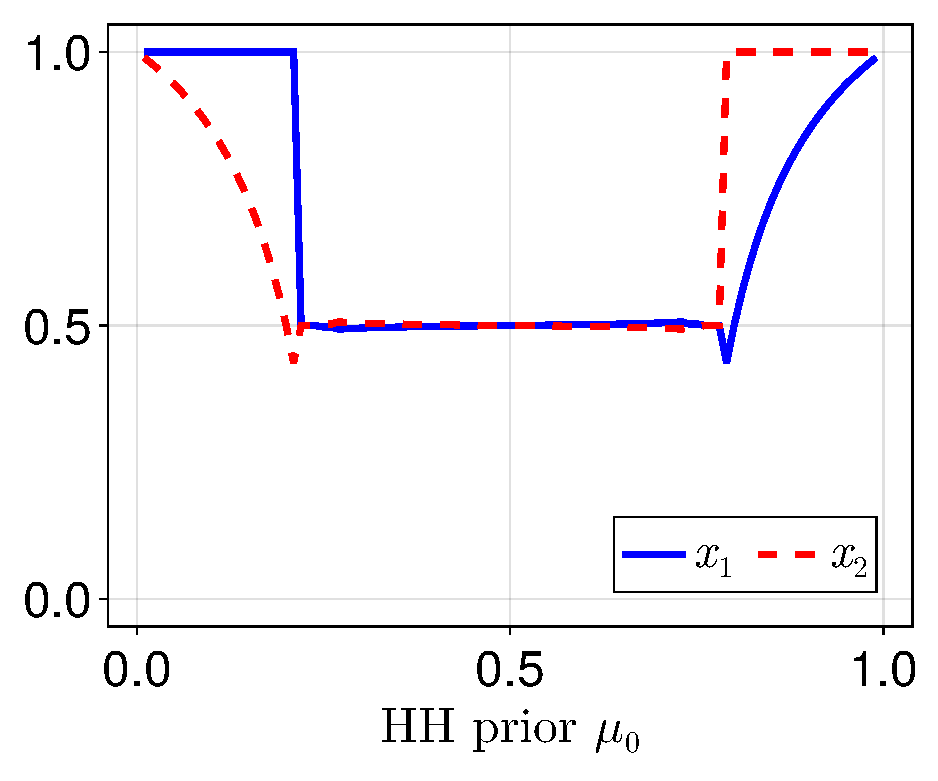
\includegraphics[width=0.49\textwidth]{figures/V8/γ_1/fig_optimal_π_across_μ_0_ω_1_1_ω_2_-1_δ_0.0_.pdf}
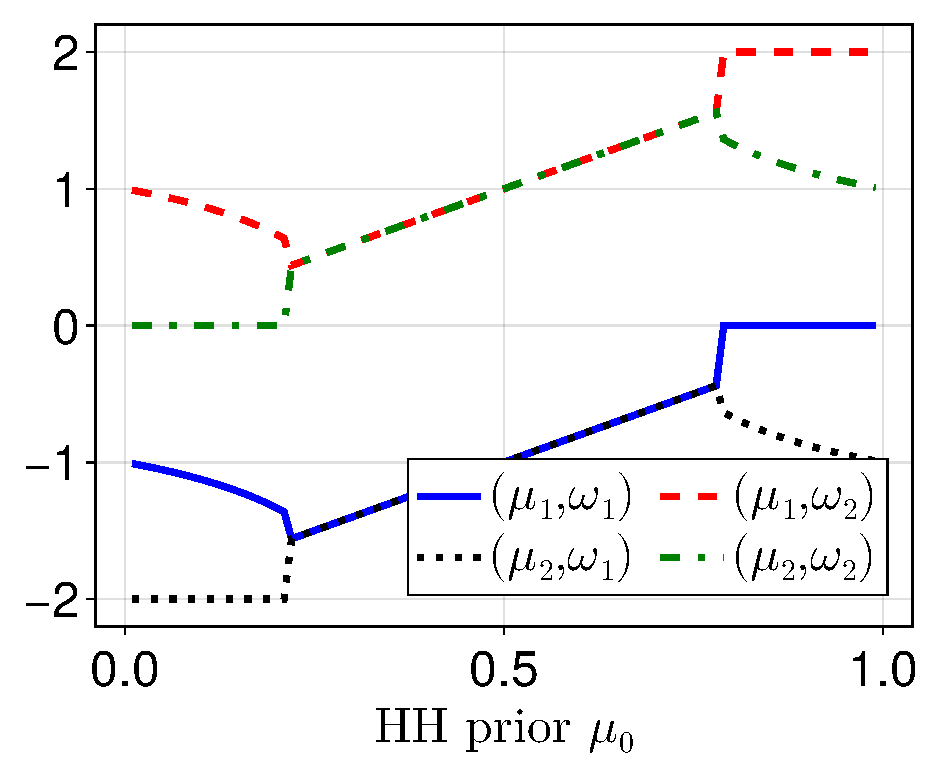
\includegraphics[width=0.49\textwidth]{figures/V8/γ_1/fig_posterior_across_μ_0_ω_1_1_ω_2_-1_δ_0.0_.pdf}
\caption{Comparative statics for $\mu_0$, when $\delta=0$, holding fixed all other parameters as in the benchmark.}
\label{FigureA21}
\end{figure}

\begin{figure}[H]
\centering
\includegraphics[width=0.49\textwidth]{figures/V8/γ_1/fig_optimal_π_across_μ_0_c_ω_1_1_ω_2_-1_δ_0.0_.pdf}
\includegraphics[width=0.49\textwidth]{figures/V8/γ_1/fig_posterior_across_μ_0_c_ω_1_1_ω_2_-1_δ_0.0_.pdf}
\caption{Comparative statics for $\mu_0^c$, when $\delta=0$, holding fixed all other parameters as in the benchmark.}
\label{FigureA22}
\end{figure}

\begin{figure}[H]
\centering
\includegraphics[width=0.49\textwidth]{figures/V8/γ_1/fig_optimal_π_across_μ_0_ω_1_1_ω_2_-1_δ_1.0_.pdf}
\includegraphics[width=0.49\textwidth]{figures/V8/γ_1/fig_posterior_across_μ_0_ω_1_1_ω_2_-1_δ_1.0_.pdf}
\caption{Comparative statics for $\mu_0$, when $\delta=1$, holding fixed all other parameters as in the benchmark.}
\label{FigureA23}
\end{figure}

\begin{figure}[H]
\centering
\includegraphics[width=0.49\textwidth]{figures/V8/γ_1/fig_optimal_π_across_μ_0_c_ω_1_1_ω_2_-1_δ_1.0_.pdf}
\includegraphics[width=0.49\textwidth]{figures/V8/γ_1/fig_posterior_across_μ_0_c_ω_1_1_ω_2_-1_δ_1.0_.pdf}
\caption{Comparative statics for $\mu_0^c$, when $\delta=1$, holding fixed all other parameters as in the benchmark.}
\label{FigureA24}
\end{figure}

\begin{figure}[H]
\centering
\includegraphics[width=0.49\textwidth]{figures/V8/γ_1/fig_optimal_π_across_μ_0_ω_1_2_ω_2_-2_δ_0.0_.pdf}
\includegraphics[width=0.49\textwidth]{figures/V8/γ_1/fig_posterior_across_μ_0_ω_1_2_ω_2_-2_δ_0.0_.pdf}
\caption{Comparative statics for $\mu_0$, when $(\delta,\omega_1,\omega_2)=(0,2,-2)$, holding fixed all other parameters as in the benchmark.}
\label{FigureA25}
\end{figure}

\begin{figure}[H]
\centering
\includegraphics[width=0.49\textwidth]{figures/V8/γ_1/fig_optimal_π_across_μ_0_c_ω_1_2_ω_2_-2_δ_0.0_.pdf}
\includegraphics[width=0.49\textwidth]{figures/V8/γ_1/fig_posterior_across_μ_0_c_ω_1_2_ω_2_-2_δ_0.0_.pdf}
\caption{Comparative statics for $\mu_0^c$, when $(\delta,\omega_1,\omega_2)=(0,2,-2)$, holding fixed all other parameters as in the benchmark.}
\label{FigureA26}
\end{figure}

\begin{figure}[H]
\centering
\includegraphics[width=0.49\textwidth]{figures/V8/γ_1/fig_optimal_π_across_μ_0_ω_1_2_ω_2_-1_δ_0.0_.pdf}
\includegraphics[width=0.49\textwidth]{figures/V8/γ_1/fig_posterior_across_μ_0_ω_1_2_ω_2_-1_δ_0.0_.pdf}
\caption{Comparative statics for $\mu_0$, when $(\delta,\omega_1,\omega_2)=(0,2,-1)$, holding fixed all other parameters as in the benchmark.}
\label{FigureA27}
\end{figure}

\begin{figure}[H]
\centering
\includegraphics[width=0.49\textwidth]{figures/V8/γ_1/fig_optimal_π_across_μ_0_c_ω_1_2_ω_2_-1_δ_0.0_.pdf}
\includegraphics[width=0.49\textwidth]{figures/V8/γ_1/fig_posterior_across_μ_0_c_ω_1_2_ω_2_-1_δ_0.0_.pdf}
\caption{Comparative statics for $\mu_0^c$, when $(\delta,\omega_1,\omega_2)=(0,2,-1)$, holding fixed all other parameters as in the benchmark.}
\label{FigureA28}
\end{figure}

\begin{figure}[H]
\centering
\includegraphics[width=0.49\textwidth]{figures/V8/γ_1/fig_optimal_π_across_μ_0_ω_1_2_ω_2_-2_δ_1.0_.pdf}
\includegraphics[width=0.49\textwidth]{figures/V8/γ_1/fig_posterior_across_μ_0_ω_1_2_ω_2_-2_δ_1.0_.pdf}
\caption{Comparative statics for $\mu_0$, when $(\delta,\omega_1,\omega_2)=(1,2,-2)$, holding fixed all other parameters as in the benchmark.}
\label{FigureA29}
\end{figure}

\begin{figure}[H]
\centering
\includegraphics[width=0.49\textwidth]{figures/V8/γ_1/fig_optimal_π_across_μ_0_c_ω_1_2_ω_2_-2_δ_1.0_.pdf}
\includegraphics[width=0.49\textwidth]{figures/V8/γ_1/fig_posterior_across_μ_0_c_ω_1_2_ω_2_-2_δ_1.0_.pdf}
\caption{Comparative statics for $\mu_0^c$, when $(\delta,\omega_1,\omega_2)=(1,2,-2)$, holding fixed all other parameters as in the benchmark.}
\label{FigureA30}
\end{figure}

\begin{figure}[H]
\centering
\includegraphics[width=0.49\textwidth]{figures/V8/γ_1/fig_optimal_π_across_μ_0_ω_1_2_ω_2_-1_δ_1.0_.pdf}
\includegraphics[width=0.49\textwidth]{figures/V8/γ_1/fig_posterior_across_μ_0_ω_1_2_ω_2_-1_δ_1.0_.pdf}
\caption{Comparative statics for $\mu_0$, when $(\delta,\omega_1,\omega_2)=(1,2,-1)$, holding fixed all other parameters as in the benchmark.}
\label{FigureA31}
\end{figure}

\begin{figure}[H]
\centering
\includegraphics[width=0.49\textwidth]{figures/V8/γ_1/fig_optimal_π_across_μ_0_c_ω_1_2_ω_2_-1_δ_1.0_.pdf}
\includegraphics[width=0.49\textwidth]{figures/V8/γ_1/fig_posterior_across_μ_0_c_ω_1_2_ω_2_-1_δ_1.0_.pdf}
\caption{Comparative statics for $\mu_0^c$, when $(\delta,\omega_1,\omega_2)=(1,2,-1)$, holding fixed all other parameters as in the benchmark.}
\label{FigureA32}
\end{figure}


% \section{Some Random Thoughts}
% It has been documented that there is greater inattention when inflation is low. Can our model rationalize this fact? 
% If the attention choice depends somehow on the magnitude of an inflation shock, I guess it's possible

\end{document}